%************************************************
\chapter{Appearance-based indoor localization: A comparison of patch descriptor performance}\label{ch:chapter4} % $\mathbb{ZNR}$
%************************************************

\section{Introduction}
\label{sec:intro}

Self-localization within an indoor space has numerous real-world 
applications, ranging from navigation inside public spaces and large shopping and social environments to
 assistive devices for people with visual impairment.   Harvesting information from 
radio-strength signals and radio beacons to perform localization is an emerging technology.  
However, few potential solutions are as compelling as those using  visual information, 
 captured from wearable or hand-held cameras, and conveyed into knowledge about how 
to navigate a space. 

\indent This work proposes an alternative approach to geometric and SLAM-based 
localization.  Location is, instead, associated through visual queries against the
 paths of other users, rather than by explicit map-building or geometric inference. 
We test this idea  in a new dataset of \emph{visual paths}~\cite{Rivera-Rubio2014}, 
containing  more than \SI{3}{km} of video sequences captured through {\em multiple} passes 
along 10 corridors  in a large building with ground truth. We compare custom-designed 
descriptors  with SIFT~\cite{Lowe2004} and HOG3D~\cite{Klaser2008}.  Standard Bag-of-Visual Words (BoVWs) approaches are used to index and associate views between journeys. The results suggest that, even without tracking, significant cues about localization can be captured and used to infer location.  The application to wearable camera technology -- whereby image cues are harvested from volunteered 
journeys, then used to help other users of the same space navigate -- is the eventual
 goal of this work, which is a natural extension to recently reported approaches based on harvesting environmental signals \cite{Wang2012}.


%We do not, for one moment, suggest that one would attempt to use vision to localize without incorporating data from other sensors that are worn, including radio signal strength, accelerometers and magnetometers.  Instead, 

%------------------------------------------------------------------------- 
\section{Related work}
\label{sec:retrieval}

\subsection{Matching between visual paths} As we briefly introduced in Chapter \ref{ch:chapter2}, we define a {\em visual path} as a collection of image frames that are induced by the relative motion of a person in a scene. The work reported in this paper involves matching the visual paths of a ``new'' journey instance to previous, similar instances. 

Early work by Matsumoto et al. \cite{Matsumoto1996} introduced a similar concept of the ``view-sequenced route representation''.  In this scheme,  a robot could perform simple navigation tasks by correlating current views against those held in a database. \citet{Ohno1996} also worked on this idea, using the difference between frames of detected vertical lines to estimate changes in position and orientation. Their results were constrained to controlled robot movement, and therefore arguably of limited applicability to images obtained from human ego-motion. Also employing vertical lines as features, this time from omni-directional images, Tang {\it et al.} used estimated position differences between sequences to perform  robot navigation \cite{Tang2001}. To make the inference more robust, they used recorded odometry at training time. This approach would certainly reduce the error in the localization task. However, it could lead to ``solving'' the training  route, without truly analysing the performance of feature matching methods. Furthermore, without ground-truth available in a crowdsensing setting, the technique of training with ground-truth is of limited usability.  On the other hand, with many passes through the same space, the reference for a journey could be the visual paths themselves. In this case, we would use ground-truth -- if available -- only to ascertain the accuracy of proposed matching or localization methods. This is the approach taken in our current work.

The performance of previously reported methods that use a retrieval-type approach, albeit of the order of tens of cm, cannot be taken as representative for the evaluation of the methods presented in this paper. The reviewed publications report results in routes of a few metres in length. Our evaluation is in a dataset three orders of magnitude longer.  Deliberately, we do not include any tracking, such as Kalman filtering, which can often hide poor measurement performance. 

\subsection{Crowdsourcing visual paths.}
Our usage setting represents a particularly data-intensive form of crowdsensing in which the image streams  from wearable cameras could be volunteered to others as reference paths for indoor journeys. An illustration of this concept is presented in Fig. \ref{fig:visualpaths}. 

This type of crowdsensing approach is gaining interest, with remarkable work from Google's indoor localization systems and crowdsourced sensor information and maps~\cite{Kadous2013}. In terms of a retrieval-based visual localization system, the NAVVIS team ~\cite{Huitl2012} released a dataset for evaluating indoor navigation from a camera-equipped robot. They also advanced earlier work on visual localization based on matching of SIFT descriptors~\cite{Park2008} to one using a bag of features that could be stored in mobile phones for quick retrieval~\cite{Schroth2011,Schroth2012}. The dataset we introduce in this work is not constrained to robot navigation, as it includes the ego-motion associated with hand-held and wearable devices.

\begin{figure}[t]
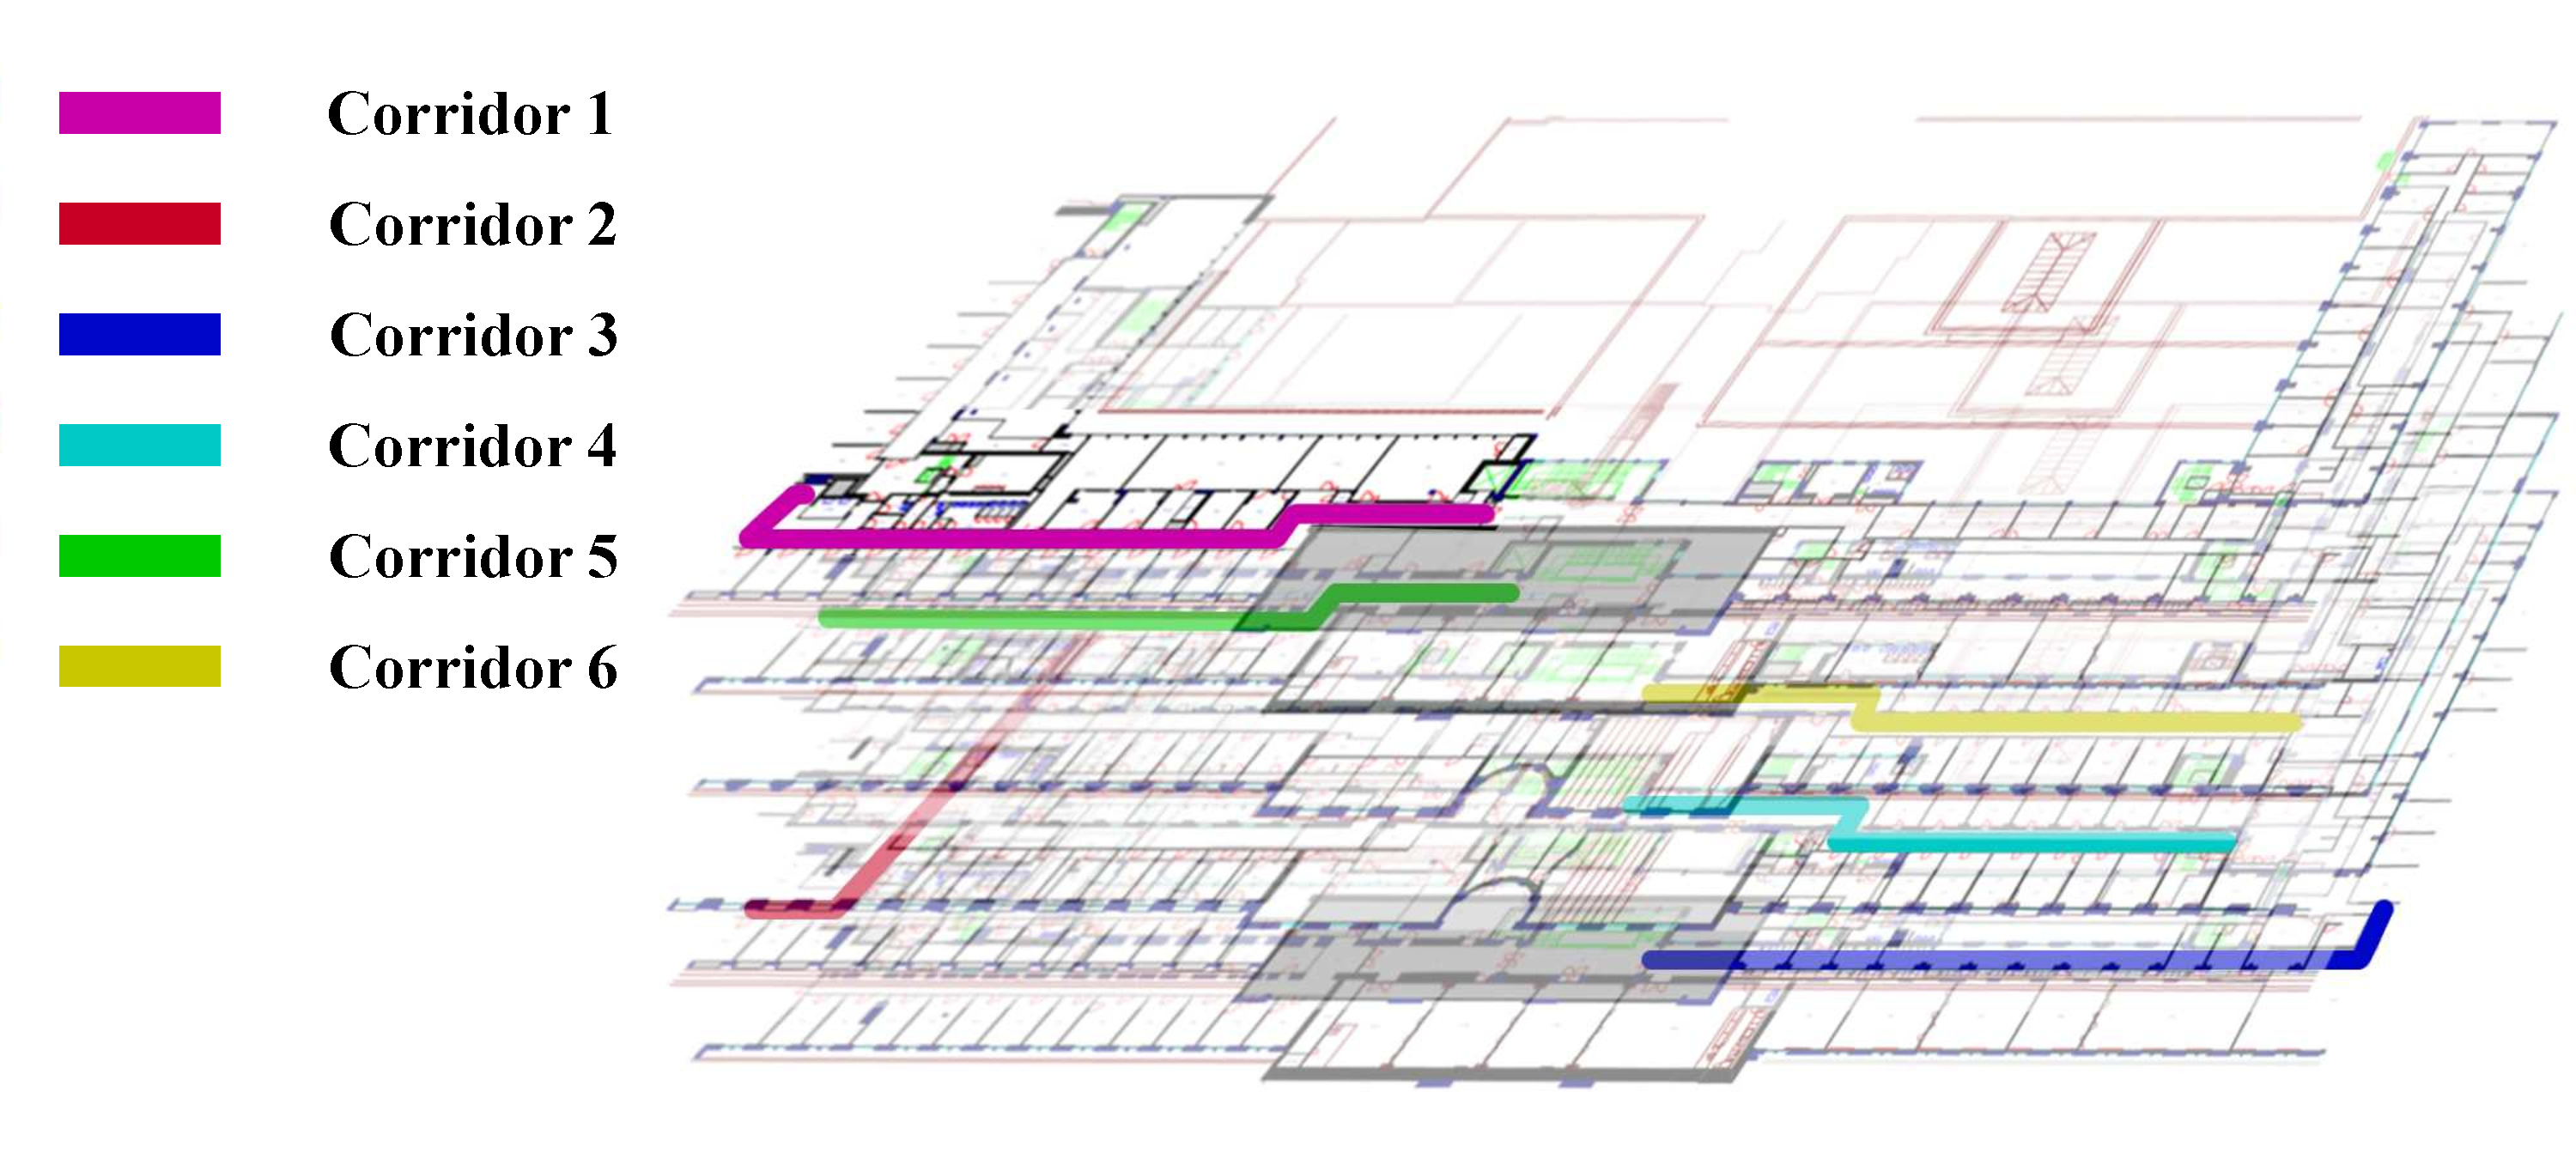
\includegraphics[width=\linewidth]{./gfx/Chapter04/map_and_legend.pdf}\label{fig:visualpathsA}
\caption{Maps of the recording locations.}
\label{fig:map_and_legend}
\end{figure}


\begin{figure}[t]

\begin{center}
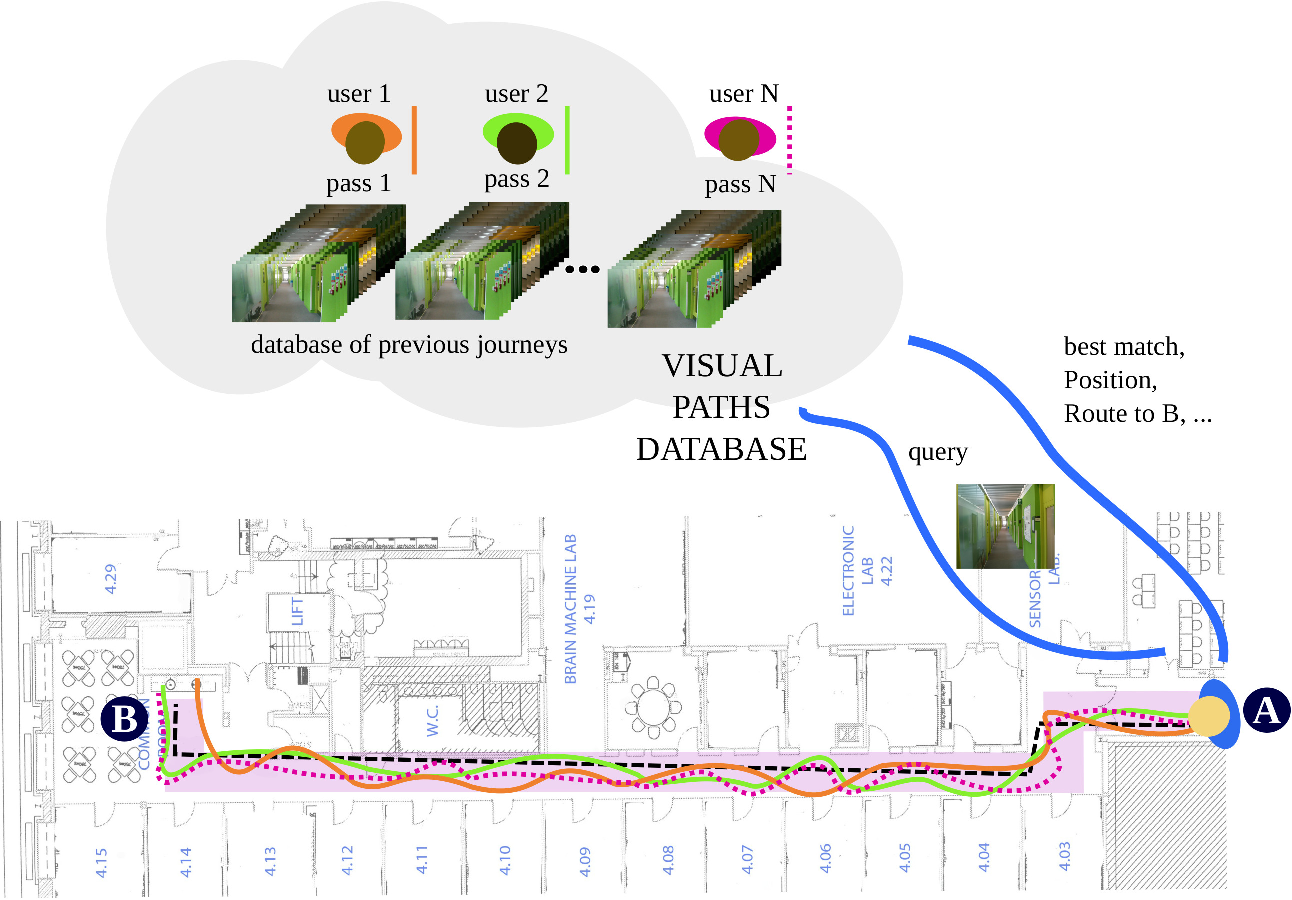
\includegraphics[width=\linewidth]{./gfx/Chapter04/corridor.pdf}
\caption{ A sample path (Corridor 1, C1) illustrating the multiple passes through the same space. Each of these passes represents a sequence that is either stored in a database, or represents the queries that are submitted against previous journeys. In the assistive context, the user at point A could be a blind or partially sighted user, and he or she would benefit from solutions to the association problem of a query journey relative to previous ``journey experiences'' along roughly the same path, crowdsourced by $N$ users that may be sighted}
\label{fig:visualpaths}
\end{center}
\end{figure}

\subsection{Alternative methods: non feature-based and sensor merging.} 
François Chaumette's team has  recently explored navigation solutions that do not require geometrical nor pixel intensities' features but use mutual information (MI) as a similarity measure. Their system performs a maximisation of the MI that is directly connected with the motion of the robot. These results, and others that rely on tracking visual features \cite{Se2002} cannot serve as a comparison for the current methods either, as they would hinder the fair evaluation of the visual features in isolation.

For outdoor navigation, the Global Positioning System (GPS) has been in widespread use for many years.  In an {\it indoor} context, localization technology is still rapidly evolving~\cite{Shen,Wang2012,Quigley2010}.  Using visual information is towards the higher end of computational complexity, and possibly the lower-end of reliability; one would certainly seek to support this approach with other forms of sensor such as Received Signal Strength Indication (RSSI) data, magnetometers, and tracking algorithms~\cite{Schroth2011,Schroth2012,Quigley2010}.  In this paper, we seek to explore efficient techniques that could be used to index and compare the visual path information gathered by multiple user journeys, and to measure the potential of vision on its own as a localization mechanism. 
%
\subsection{A biological intuition.} Another source of our motivation for the idea of retrieval-based localization is supported by the well-characterized biological hippocampal place cells~\cite{burgess2002human} that recognise a location from sensory inputs that include those captured by an animal's eyes. This does {\it not} suggest that techniques based on optical flow are not relevant: rather, the striking conclusion from recent research is that multiple approaches to visual location inference are at work in biological systems, including optic flow~\cite{Layton2014}, and other mechanisms that may not explicitly involve brain areas specialized in visual motion computation~\cite{Hartley2014space}. We will link the findings of the present chapter with this biological intuition in Chapter \ref{ch:chapter5}, where we will propose a model of the hippocampal place cells for indoor localization.


%------------------------------------------------------------------------- 
\section{Methods}
\label{sec:methods}

In this section we describe the different image description modalities we have evaluated, starting by the feature extraction process, followed by the descriptor quantization and distance metric used.

\subsection{Pipeline}

We evaluated the performance of several approaches to matching image queries taken from one visual path against the remainder of the visual paths.  In order to index and query the visual path datasets, we adopted a sequence of processes that is illustrated in Fig. \ref{fig:FigPipeline}.  We describe the details behind each of the processes (\eg gradient estimation, spatial pooling) in Section \ref{sec:descriptors}.  We considered descriptors that operate on {\em single} frames (spatial) as well as descriptors that operate on {\em multiple} frames (spatio-temporal).

\begin{figure}
\begin{center}
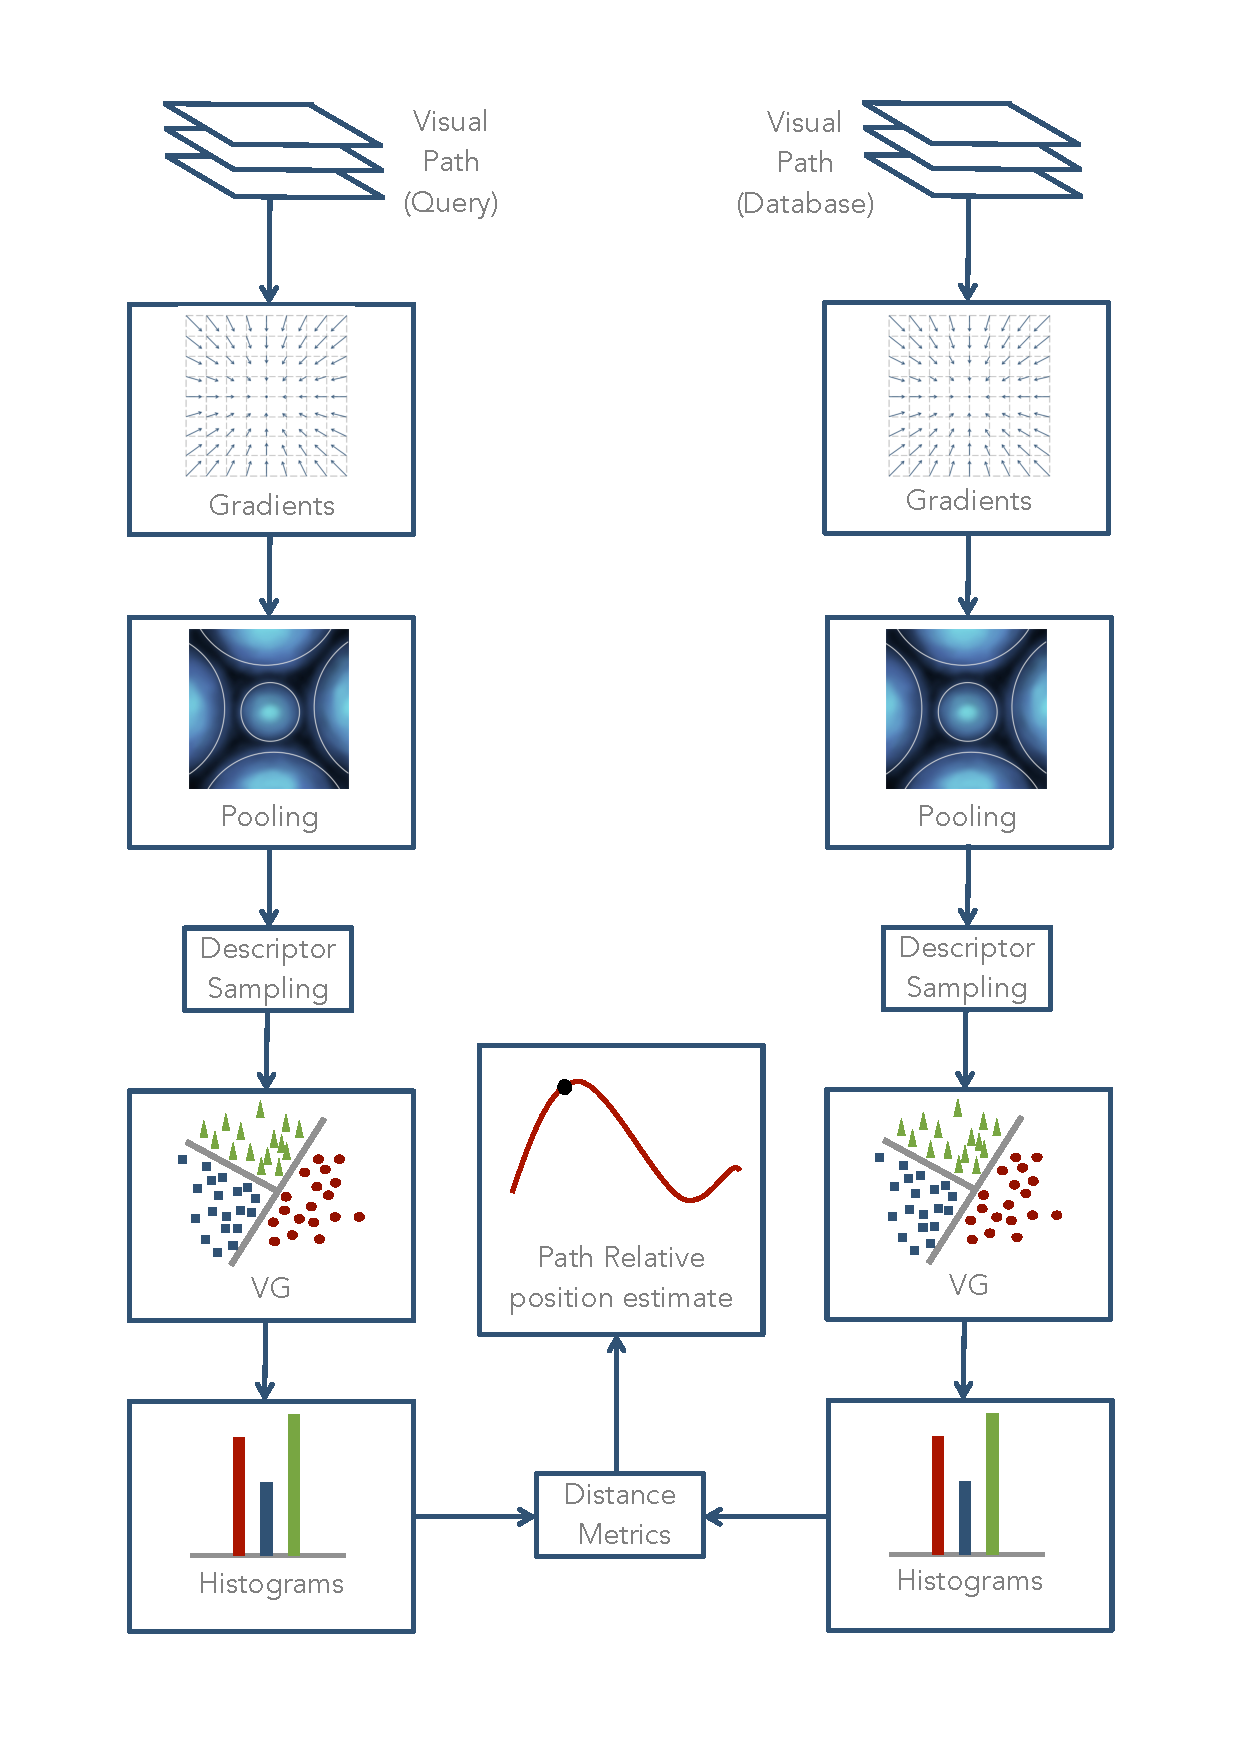
\includegraphics[width=\textwidth]{./gfx/Chapter04/pipeline.pdf}
\caption{The stages in processing image sequences from database and query visual paths are illustrated above.  This does not show the process behind the estimation of ground-truth for the experiments, which is described separately in Section \ref{sec:exp_methods}.  Variants of the gradient and pooling operators, quantization approaches and distance metrics are described in Section \ref{sec:methods}.}
\label{fig:FigPipeline}
\end{center}
\end{figure}

\subsection{Frame-Level Descriptor}
Based on the use of optical flow in motion estimation~\citep{Weickert2006} and space-time descriptors in action recognition \citep{Wang2009} we estimated in-plane motion vectors using a simple approach.  We first applied derivative filters along $(x,y,t)$ dimensions, yielding a 2D$+t$, i.e. spatio-temporal, gradient field.  To capture variations in chromatic content from the visual sequence, we computed these spatio-temporal gradients separately for each of the three RGB channels of the pre-processed video sequences.  This yielded a $3\times 3$ matrix at each point in space.  Temporal smoothing was applied along the time dimension, with a support of 11 neighbouring frames. Finally, the components of the matrix were each averaged (pooled) over 16 distinct spatial regions, not very dissimilar to those to be described later in this paper.   For each visual path, this yielded 144 signals, of length approximately equal to the video sequences.  An illustration of the time series for one visual path is shown in Fig.~\ref{fig:Traces}.

\begin{figure}
\begin{center}
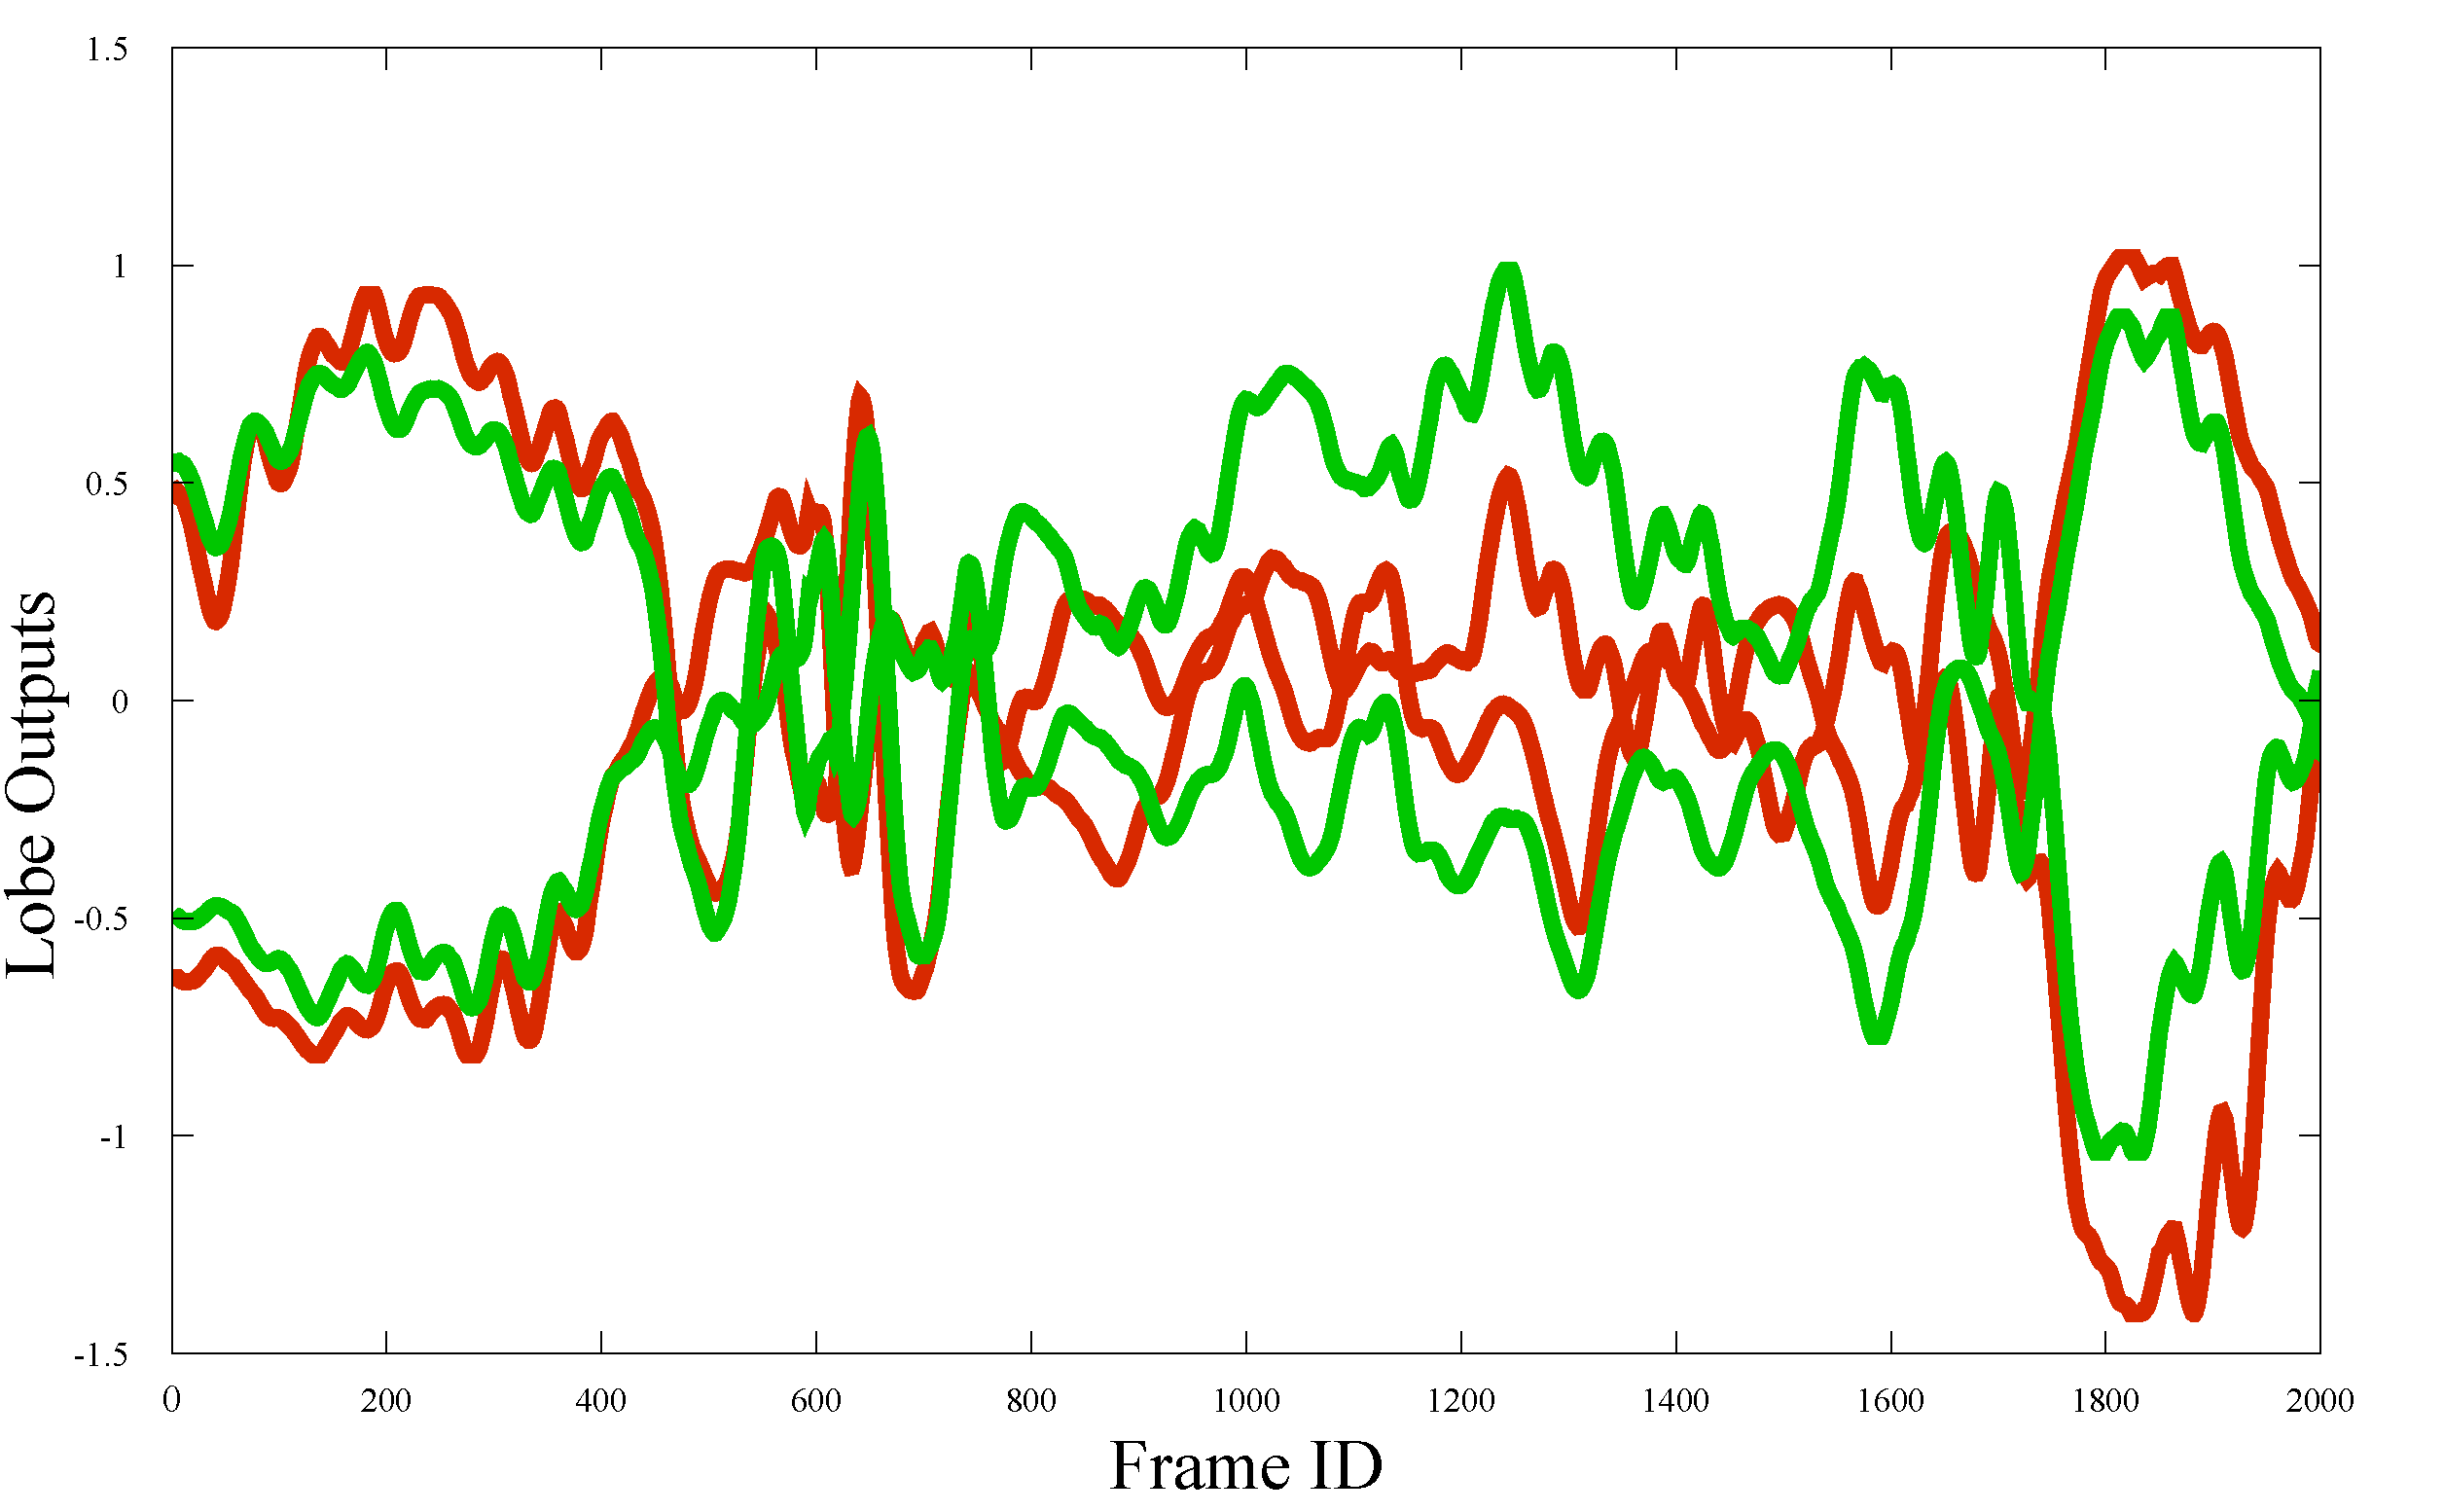
\includegraphics[width=\linewidth]{./gfx/Chapter04/Lobe1and6_red_green.pdf}
\caption{Four (of 144) representative signals acquired from a visual path; these signals encode changes in red and green channels as a user moves through space.  The collection of signal traces at one point in time can be used to build a simple frame-level space-time descriptor: LW\_COLOR. The signal amplitudes are spatially pooled temporal and spatial gradient intensities.}
\label{fig:Traces}
\end{center}
\end{figure}

At each point in time, the values over the 144 signal channels are also captured into a {\it single} space-time descriptor per frame: 
LOR.  Our observations from the components of this descriptor are that a) relative ego-motion is clearly identifiable in the signals; b) stable patterns of motion may also be identified, though changes in the precise trajectory of a user could also lead to perturbations in these signals, and hence to changes in the descriptor vectors. Minor changes in trajectory might, therefore, reduce one's ability to match descriptors between users.  These observations, together with the possibility of partial occlusion, led us to the use of {\em patch} based descriptors, so that multiple descriptors would be produced for each frame. These are introduced next.


\subsection{Local descriptors}
\label{sec:descriptors}

\paragraph{Keypoint based SIFT (KP\_SIFT).}

The original implementation of Lowe's SIFT descriptor follows the extraction of interesting points in the image that are stable to certain transformations, the ``SIFT keypoints'' \cite{Lowe2004}. This is widely used across many branches of computer vision, from object recognition to motion detection and SLAM. We used the standard implementation from VLFEAT \cite{Vedaldi2008} to compute $\vec{\nabla}f(x,y;\sigma)$ where $f(x,y;\sigma)$ represents the embedding of image $f(x,y)$ within a Gaussian scale-space at scale $\sigma$. We set the parameter \emph{PeakThresh} to 0 to filter out small local maxima in scale-space.

\paragraph{Dense SIFT (DSIFT).}

The Dense-SIFT (DSIFT) descriptor \citep{Lazebnik2006} is a popular  alternative to keypoint based SIFT. It sacrifices some invariance properties available with keypoint-based SIFT, producing descriptors that are densely, rather than sparsely, distributed across the image. This DSIFT descriptor was calculated by  sampling of the smoothed estimate of $\vec{\nabla}f(x,y;\sigma)$.  We used the implementation of the VLFEAT toolbox, setting $\sigma = 1.2$, with a stride length of 3 pixels. This  yielded around $2,000$ descriptors per frame, each describing a patch of roughly $10 \times 10$ pixels.  \\

\paragraph{Single Frame Gabor descriptors (SF\_GABOR).}

An alternative single frame technique based on a tuned, odd-symmetric Gabor-based descriptor is the SF\_GABOR. For this, we used $8$-directional spatial Gabor filters previously tuned on PASCAL VOC data \cite{Everingham2009} in order to provide an implicit encoding of the orientation of local image structures.  Each filter gives rise to a filtered image plane, denoted $\mathbf{G}_{k,\sigma}$.  For each plane, we compute the discrete spatial convolution, $\mathbf{G}_{k,\sigma} \ast {\Phi}_{m,n}$, with a series of pooling functions, ${\Phi}_{m,n}$. The latter are produced by spatial sampling of the function:

\begin{equation}
\Phi(x,y;m,n) = e^{-\alpha \left [\log_e \left ( \frac{x^2+y^2}{d_n^2}\right ) \right ]^2 - \beta |\theta-\theta_m | }
\label{eq:pool1}
\end{equation}

\noindent with $\alpha = 4$ and $\beta = 0.4$. The values of $m$ and $n$ were chosen to produce 8 angular regions at each of two distances $d_1, d_2$ away from the centre of a spatial pooling region.  For the central region, corresponding to $m=0$, there was no angular variation but instead a log-normal radial decay, with a limiting value at $(x,y)=(0,0)$. This arrangement yielded a total of  17 spatial pooling regions. The resulting $17 \times 8$ fields are sub-sampled to produce dense 136-dimensional descriptors, each representing an approximate $10 \times 10$ region, and yielding around 2,000 descriptors per image frame after spatial sub-sampling. 

\begin{figure}[t]
\centering
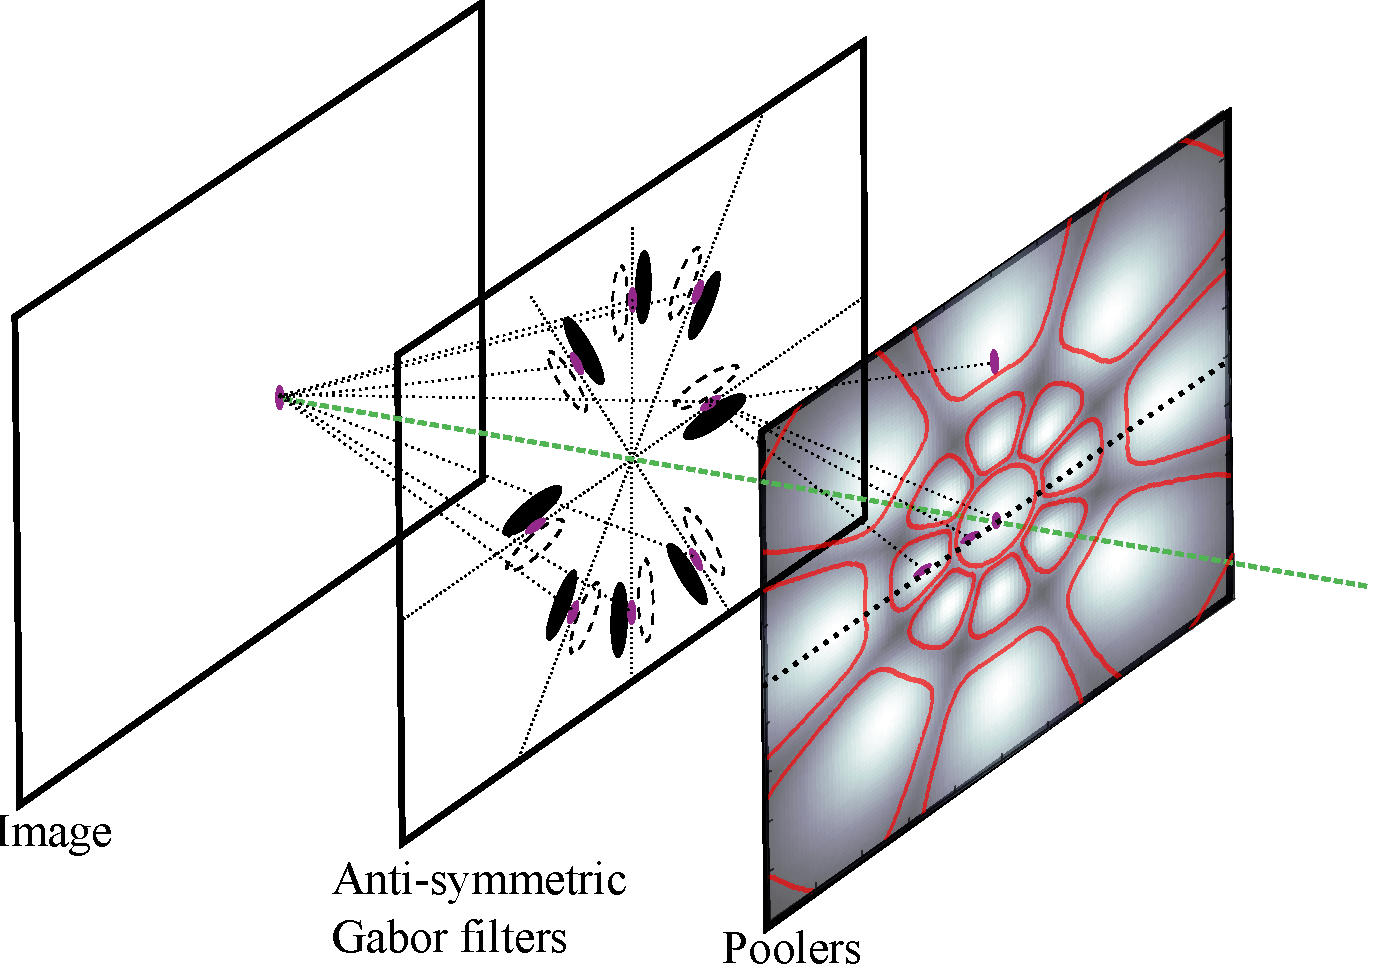
\includegraphics[width=0.7\linewidth]{./gfx/Chapter04/Layers.pdf}
\caption{The spatial pooling pattern used for single frame Gabor filtering is based on the regions shown here.  These regions were generated by sampling Eq.~(\ref{eq:pool1}) to create pooling masks. The masks can be applied to the Gabor filtered video frame outputs by spatial convolution, followed by sub-sampling the output every 3 pixels. See text for further details.}
\label{fig:IsoPool}
\end{figure}

\paragraph{Space-Time descriptors.}
%We therefore chose to explore a denser sampling of the image through capturing patterns over space-time patches in a dense fashion.  We tried three approaches to achieve this.  These are a) the HOG3D descriptor from \cite{Klaser2008}; and two novel techniques, one b) based on antisymmetric Gabor functions of space and time; and one c) incorporating smoothing in time, and gradients in space.  These approaches are somewhat similar to that described in Section \ref{sec:ODPF}, in the sense of using spatial derivatives and incorporating information across time, increasing description accuracy at the expense of computational load (see Table~\ref{table:comput_load}).  A further point to note is that the methods in this section do not make use of colour, using grey-scale information only from the intensity channel of HSI space. Although discarding an important potential visual cue of location, this allowed us to compare performance against a previously described method of HOG3D, providing some confidence that the new techniques are at least comparable to methods already in use.  
%
%The three approaches described in this section require two additional processes. First, an explicit calculation of the direction of the space-time, or gradient vector, that encodes visual motion is carried out.  Secondly, to reduce the information obtained from a dense collection of descriptors so as to make frame-by-frame query possible, a dictionary-learning approach was taken to map descriptors to atoms, then to map atoms to histograms for the database and queries.  This increased complexity does not greatly affect run-time queries when efficiently implemented, but does contribute to on-line vocabulary building and encoding in order to enable efficient performance at query time.
%
%\subsubsection{The HOG3D Descriptor}
%The 3D gradient estimation on the HOG3D feature is done by applying derivative filters along the three main dimensions of the video $(x,y,t)$. The resultant gradient vector is projected to unit vectors in a 3D quantised space (20 faces of an icosahedron). Similar to the HOG3D features, an odd symmetric Gabor filter is used on each video dimension to compute the 3D gradient vector. Projection to 12 directions in 3D space (dodecahedron) is used to quantise the motion vector in space-time. From this, a descriptor is produced.  We used the author's implementation, described in \cite{Klaser2008}.
%
%\subsubsection{Spatio-Temporal Gabors (ST\_GABOR)}
%Spatio-temporal Gabors have been used in activity recognition, and in structure from motion.  In what might be considered ``location from motion'', we performed one-dimensional convolution $(\ast)$ between the intensity video-sequence $I(x,y,t)$ and antisymmetric, one-dimensional Gabor functions of space, $x,y$, and time, $t$, respectively:
%\begin{equation}
%\begin{array}{c}
%I_1(x,y,t) = I(x,y,t) \ast g_x(x;\sigma_x) \\
%
%I_2(x,y,t) = I(x,y,t) \ast g_y(y;\sigma_y) \\
%
%I_3(x,y,t) = I(x,y,t) \ast g_t(t;\sigma_t)
%
%\end{array}
%\label{eq:convolutions}
%\end{equation}
%
%The parameters of $\sigma_x$ and $\sigma_y$ were set to be equal, and to provide one complete cycle over approximately 5 pixels of spatial extent. For the temporal operator, $\sigma_t$ was set to provide temporal support of 9 pixels, and included one complete cycle of oscillation.  We used anti-symmetric Gabor functions, as they were found to perform better than symmetric functions in our data.
%
%The components $(I_1,I_2,I_3)$ now represent each pixel in each frame in a three-dimensional feature space. Magnitude-weighted votes are then placed into the two bins corresponding to the elevation and azimuthal angles, respectively, of this feature vector.   The information in these bins is then collected within each of 17 lobes over a fairly small patch size of $16\times 16$ pixels in spatial extent in a single reference frame at the centre of the temporal support region.   These lobes were similar to those shown in Fig. ~\ref{fig:kernel}, with one additional central lobe, and used a spatial weighting pattern similar to the DAISY descriptor \cite{Winder2009}.  The resulting descriptor, produced for each patch of image space, is only slightly larger than that based on the colour descriptor described in Section \ref{sec:ODPF}.  However, the descriptors are computed {\it densely} over space, by sampling patches across the image on a regular grid.  Thus, just over 2000 of these 192-dimensional descriptors are produced per frame.
%
%\subsubsection{Spatial Derivative, Temporal Gaussian (ST\_GAUSS)}
%A final variant of descriptor was designed. In this case, we tried smoothing in time, rather than taking a derivative, then computing simple derivatives over space using a pair of directional derivative-of-Gaussian spatial filters of size ($5\times 5$). The temporal smoothing was provided by an 11-point Gaussian smoothing filter with a standard deviation of 2.  This was applied before the two dimensional spatial-derivative masks.
%Once the gradient field was estimated, the gradient direction was calculated and quantised into 4 directions, with a sign calculation being used to generate 8 directions.  A simple Parzen-type operation smoothed the angles into a weighted histogram of spatial orientations.
%The descriptor was then constructed by using pooling regions that are very similar to those described above, yielding a 192-dimensional histogram. Finally, the patches of each frame were densely sampled, to produce around 2000 descriptors per frame.


Given the potential richness available from space-time information, we explored three distinct approaches to generate space-time patch descriptors.  When generating the descriptor associated with each patch, all  approaches yield multiple descriptors per frame, and all take into account neighbouring frames in time.  In contrast to a sparse-sampling approach of a keypoint-based descriptor, all three densely sample the video sequence.  The three methods are i) HOG 3D~\cite{Klaser2008}; ii) a space-time, antisymmetric Gabor filtering process (ST\_GABOR); and iii) a Spatial Derivative, Temporal Gaussian (ST\_GAUSS) filter.\\

\begin{enumerate}
\item The \textbf{HOG 3D} descriptor (HOG3D) \citep{Klaser2008} was introduced with the aim of extending the very successful two-dimensional histogram of oriented gradients technique \citep{Dalal}, to space-time fields, in the form of video sequences.  HOG 3D seeks computational efficiencies by smoothing using box filters, rather than Gaussian spatial or space-time kernels.  This allows three-dimensional gradient estimation across multiple scales using {\em integral video} representations, a direct extension of the integral image idea \citep{Viola2001}.  The gradients from this operation are usually performed across multiple scales.  We used the dense HOG 3D option from the implementation of the authors, and the settings yielded approximately 2,000  descriptors per frame of video. Each descriptor contained 192 elements.

\item \textbf{Space-time Gabor (ST\_GABOR)} functions have been used in activity recognition, structure from motion and other applications \cite{Bregonzio2009}.  We performed one dimensional convolution between the video sequence and three one-dimensional Gabor functions along either one spatial dimension i.e.\ $x$ or $y$, or along $t$.  The one-dimensional convolution  is crude, but appropriate if the videos have been downsampled. The spatial extent of the Gabor function was set to provide one complete cycle of oscillation over approximately 5 pixels of spatial span, both for the $x$ and $y$ spatial dimensions. The filter for the temporal dimension was set to provide  around one oscillation over 9 frames.  We also explored symmetric Gabor functions, but found them rather less favourable.

After performing three separate filtering operations, each pixel of each frame is assigned a triplet of values corresponding to the result of each filtering operation.  The three values are treated as being components of a 3D vector.  Over a spatial extent of around $16 \times 16$ pixels taken at the central frame of the 9-frame support region, these vectors contribute weighted votes into descriptor bins according to their azimuth and elevations, with the weighting being given by the length of the vector.  The votes are also partitioned according to the approximate spatial lobe pattern illustrated in Fig.~\ref{fig:IsoPool}. Each frame had approximately 2,000 ST\_GABOR descriptors, each of 221 elements.


\item A final variant of space-time patch descriptor was designed.  This consisted of spatial derivatives in space, combined with smoothing over time \textbf{(ST\_GAUSS)}.  In contrast to the strictly one-dimensional filtering operation used for the ST\_GABOR descriptor, we used two $5\times 5$ gradient masks for the $x$ and $y$ directions based on derivatives of Gaussian functions, and an 11-point Gaussian smoothing filter in the temporal direction, using a standard deviation of 2.  8-directional quantization was applied to the angles of the gradient field, and a voting process incorporating gradient magnitude was used to distribute votes across the bins of a 136-dimensional descriptor.  Like the ST\_GABOR descriptor, pooling functions, similar to those shown in Fig.~\ref{fig:IsoPool}, were applied.  The number of descriptors produced was the same as for the other methods using patch-level descriptions.
\end{enumerate}


\subsection{Quantization and histogram encoding}

Our initial conjecture was that whole frames from a sequence could be indexed compactly, using the single-frame descriptor (LW\_COLOR).  This was found to lead to disappointing performance (see Section~\ref{sec:ch4results}). For the case of many descriptors-per-frame i.e.\ descriptors that are patch-based, we have the problem of generating around 2,000 descriptors per frame, if dense sampling is used.  Thus, we applied vector quantization (VQ) to the descriptors, then used histograms of VQ descriptors, effectively representing each frame as a histogram of words \citep{Csurka2004}. The dictionary was always built by excluding the entire journey from which queries are to be taken.  

The resulting dictionaries were then used to encode the descriptors of the $M-1$ training passes and the remaining query pass. Two different approaches to the encoding of descriptors were taken, one based on standard $k$-means, using a Euclidean distance measure (hard assignment, ``HA''), and one corresponding to the Vector of Locally Aggregated Descriptors (VLAD) \citep{jegou2010aggregating}. These histograms were all $L_2$-normalised.  

In the HA case, the dataset was partitioned by selecting $M-1$ of the $M$ video sequences of passes through each possible path. These $M-1$ sequences have a total of $N$ frames. A dictionary of visual words was created by running the $k$-means algorithm on the partitioned set of training descriptors contained in the $N$ frames.   We fixed the dictionary size to 4,000 in order to achieve a balance between computational time and atom stability, and allowing comparison with the work of others \cite{Chatfield2011}.

For VLAD, a $k$-means clustering was first performed using a dictionary size of 256 words. For each descriptor, sums of residual vectors were used to improve the encoding.  Further advances to the basic VLAD, which include different normalizations and multiscale approaches, are given by \cite{Arandjelovic}. 

\subsection{Localization using histogram distances}
\label{sec:kernel_encodings}
Once histograms had been produced, a distance measurement was used to compare the similarity of histograms in a query frame with the database entries.  The query operation was simply performed by using the kernel approaches described in \cite{Vedaldi2010}.  Concretely, to compare encodings, either $\chi^2$ or Hellinger distance metrics \citep{Vedaldi2012} were used to retrieve results for HA and VLAD encoding approaches respectively. Distance comparisons were performed directly between either hard assigned Bag-of-Words (BoW) or VLAD image encodings arising from collections of descriptors for each frame. For the $M-1$ videos captured over each path in the database, the queries were constructed from the remaining path.   Each query frame, $H_q$, resulted in $M-1$ separate comparison vectors containing scores.  By using these kernel-based comparisons (which are always positive, and act as the inverse of a distance metric), we identified the best matching frame, $\hat{f}$, from pass, $\hat{p}$, across all of the $M-1$ vectors.  This may be expressed as: 
\begin{equation}
L(\hat{p},\hat{f}) = \underset{p,f}{\textrm{argmax}} \lbrace K_{D}(H_q,H_{p,f})\rbrace
\label{eq:argmax}
\end{equation}
where $H_{p,f}$ denotes the series of normalised histogram encodings, indexed by $p$ drawn from the $M-1$ database passes, and $f$ denotes the frame number within that pass. $K_D$ denotes the so-called ``kernelized'' version of distance measure \cite{Vedaldi2010}.  To measure the localization error, we used the ground-truth estimates that were acquired at the same time as the videos. The estimated position of a query, $L$, was simply taken to be that of the best match given by Eq. (\ref{eq:argmax}).  However, in a more robust implementation, checks could be done that would require similar matches in neighbouring frames, both in query and pass.
%%END EDIT BLOCK


%------------------------------------------------------------------------- 
\section{Experiments}
\label{sec:exp_methods}

\subsection{Data acquisition and ground truth}
\label{sec:Dataset}

A total of 60 videos were acquired from 6 corridors of a large building.  Two different devices were used for the acquisition, with 30 videos each. One was an LG Google Nexus 4 phone running Android 4.4.2.  The video data was acquired at approximately 24-30 fps at two different resolutions, $1280 \times 720$ and $1920\times 1080$ pixels.  Google Glass (Explorer edition) was used at a resolution of $1280 \times 720$, at a frame rate of 30 fps.  A surveyor's wheel (Silverline) with a precision of 10 cm and error of $\pm 5\%$ was used to record distance, but was modified by wiring its encoder to a Raspberry Pi running a number of measurement processes.  The Pi was synchronised to network time, enabling synchronisation with timestamps in the video sequence.  Because of the variable-frame rate of acquisition, timestamp data from the video was used to align ground-truth measurements with frames. This data was used to assess the accuracy of associating positions along journeys through frame indexing and comparison.

The dataset contains 3.05 km of journey data acquired at a casual indoor walking speed.  For each corridor, ten passes (i.e.\ 10 separate visual paths) were obtained. Five of these videos were acquired with the hand-held Nexus, and the remainder with Glass.  Table~\ref{tbl:Datasets} summarises the acquisition.  The length of the sequences varies, due to a combination of different walking speeds and/or different frame rates and corridor lengths. A combination of daylight/nighttime acquisitions was also performed, and prominent windows occasionally introduced strong lighting in some portions of the videos.  Variations are observable in some of the corridors from one pass to another, due to physical changes and occasional appearances from people walking along. In total, more than 90,000 frames of video were labelled with positional ground-truth in a path-relative fashion. The dataset is publicly available  at \citep{Rivera-Rubio2014} (\url{http://rsm.bicv.org}).

\begin{figure}[t]
\centering
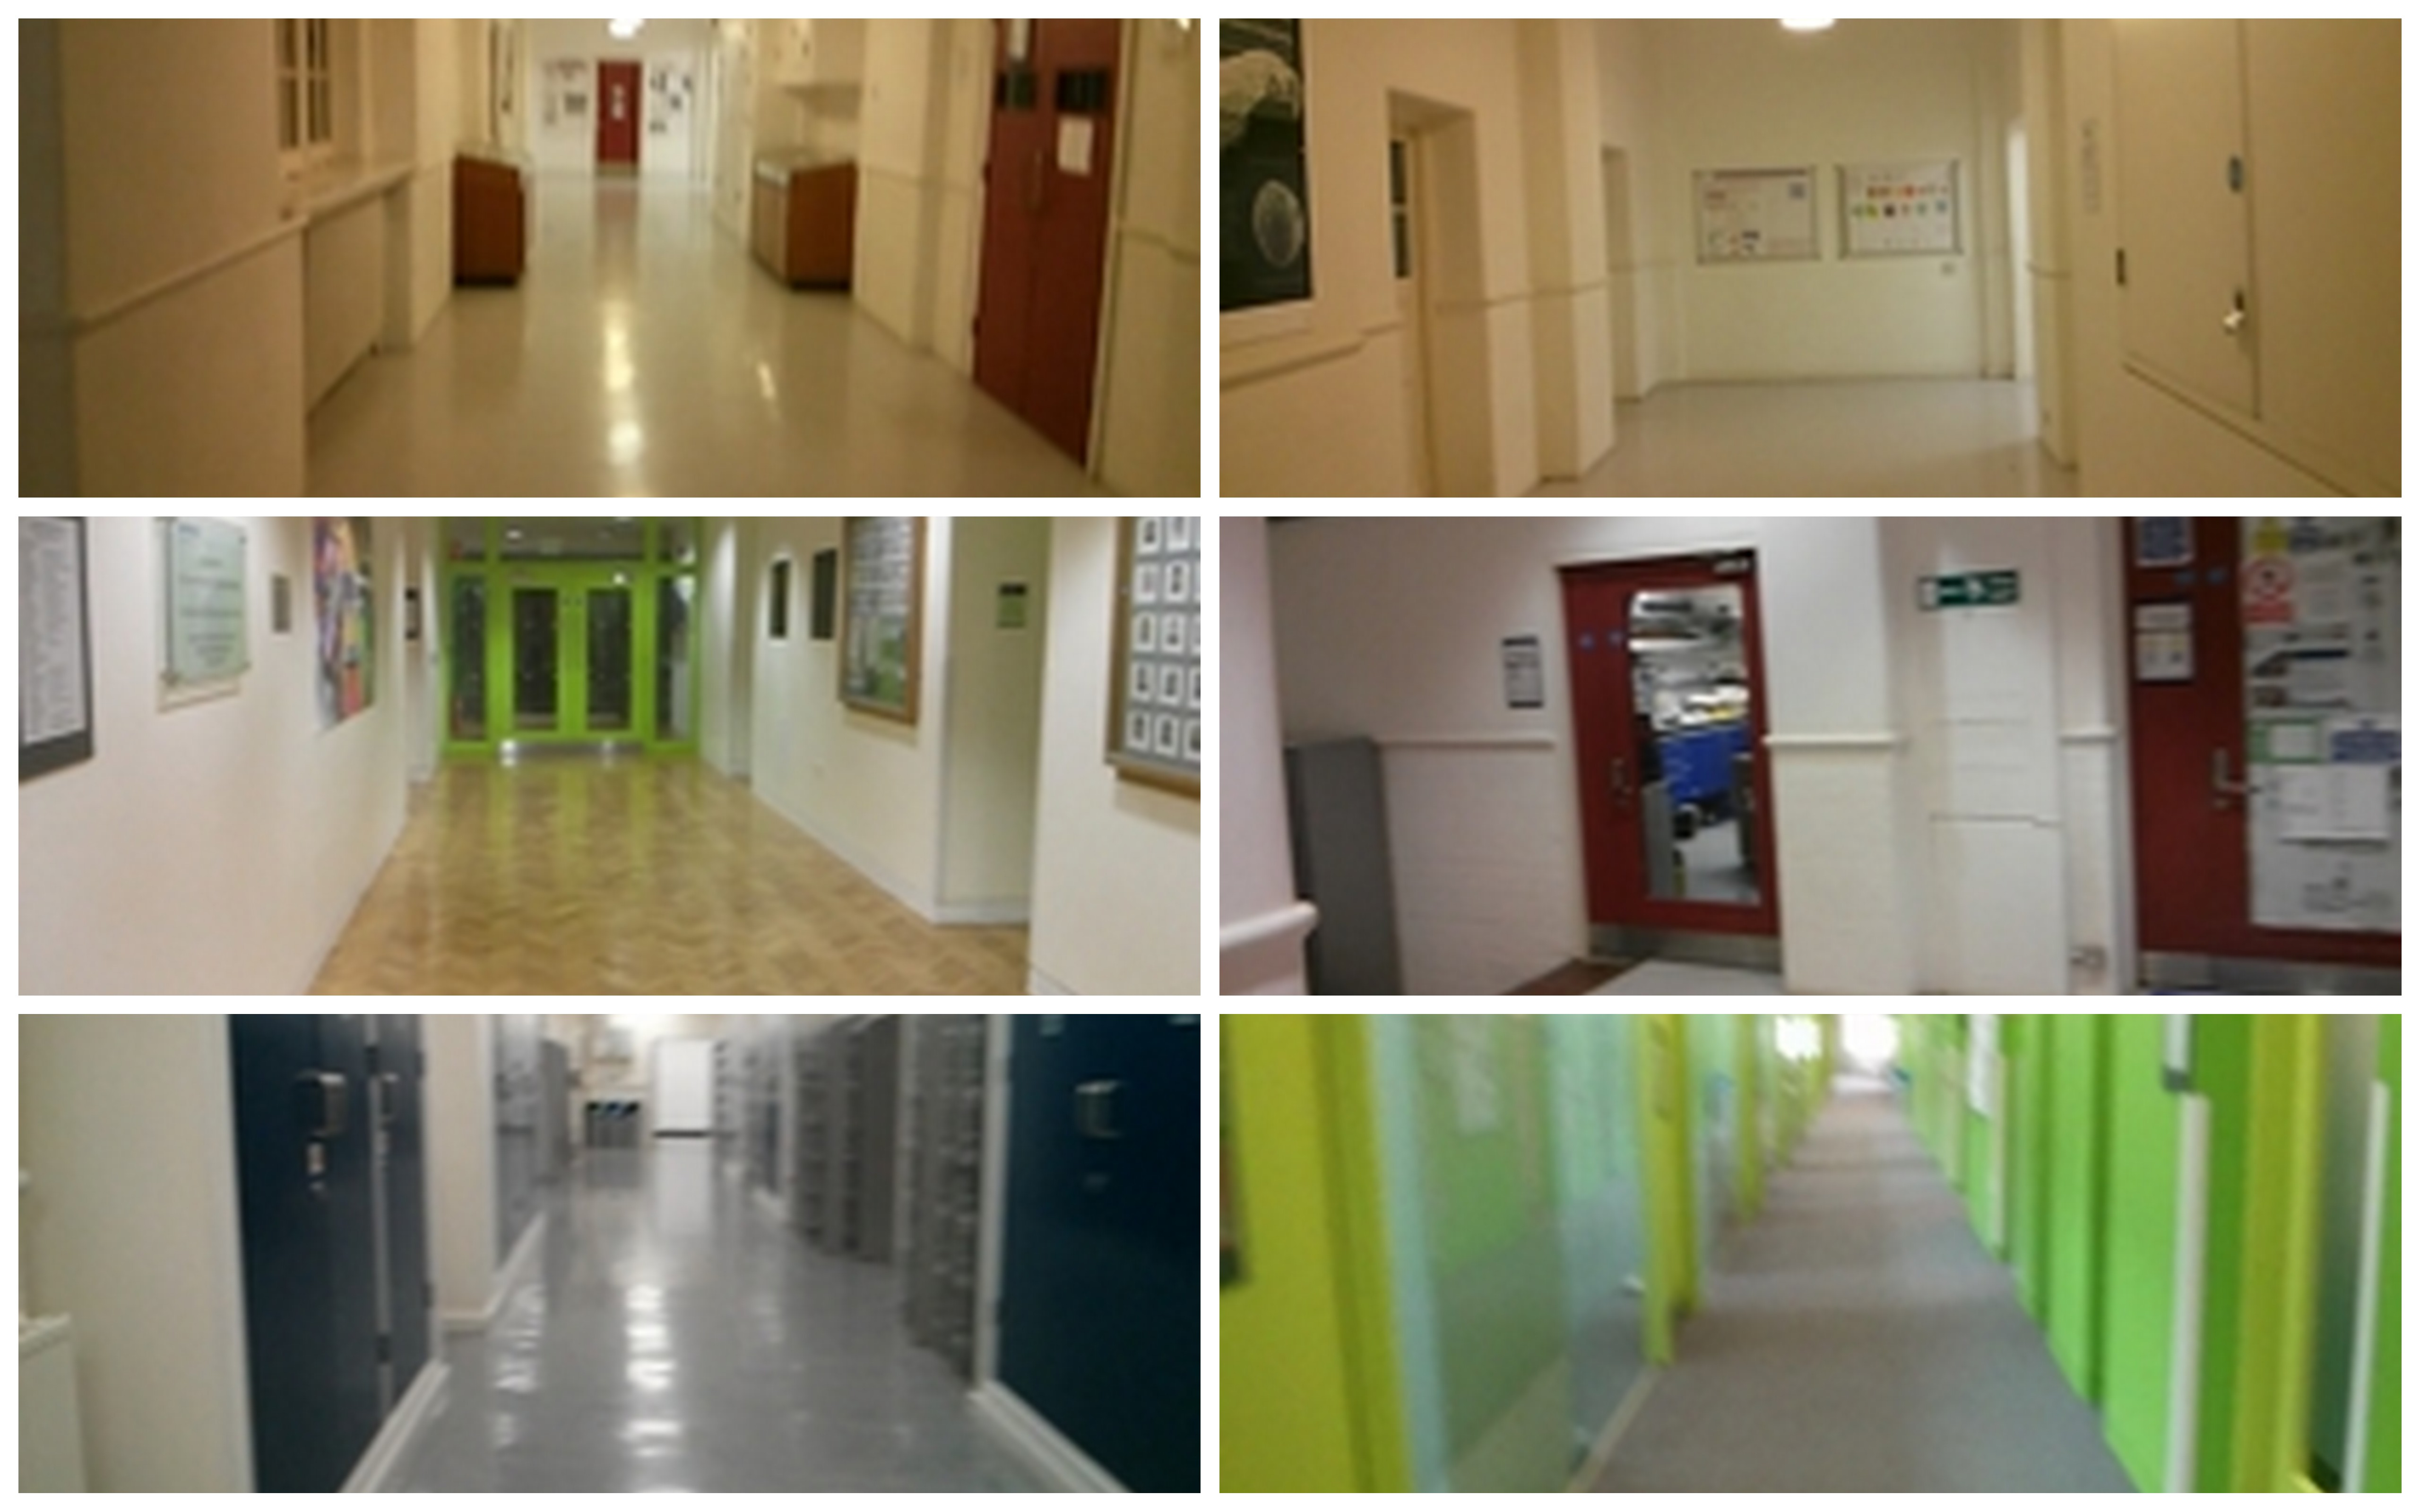
\includegraphics[width=\linewidth]{./gfx/Chapter04/rsm_collage.jpg}
\caption{A ``collage'' depicting a thumbnail of each corridor of the RSM dataset. From top left to bottom right C1, C2, ..., C6.}
\label{fig:IsoPool}
\end{figure}


\begin{table}[ht]
\caption{A summary of the dataset with thumbnails}
\label{tbl:Datasets}

\begin{center}

\centering
    \begin{tabular}{l c c c c c c c}
    \hline
    & \multirow{2}{*}{\bf{Photo}} & \multicolumn{3}{c}{\bf{Length (m)}} & \multicolumn{3}{c}{\bf{No. of frames}}  \\ \cline{3-8}
             & ~     & Avg    & Min   & Max   & Avg              & Min  & Max  \\ \hline
    C1       & \begin{minipage}{.1\textwidth}
      			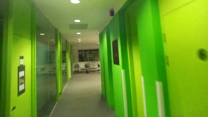
\includegraphics[width=\linewidth]{./gfx/Chapter04/table/1.jpg}
			   \end{minipage}
			        & 57.9  & 57.7 & 58.7 & 2157         & 1860 & 2338 \\ \hline
    C2       & \begin{minipage}{.1\textwidth}
      			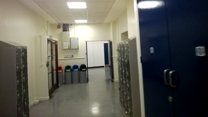
\includegraphics[width=\linewidth]{./gfx/Chapter04/table/2.jpg}
			   \end{minipage}
         & 31.0  & 30.6 & 31.5 & 909          & 687  & 1168 \\ \hline
    C3       & \begin{minipage}{.1\textwidth}
      			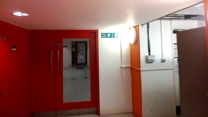
\includegraphics[width=\linewidth]{./gfx/Chapter04/table/3.jpg}
			   \end{minipage}
			        & 52.7  & 51.4 & 53.3 & 1427         & 1070 & 1777 \\ \hline
    C4       & \begin{minipage}{.1\textwidth}
      			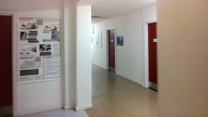
\includegraphics[width=\linewidth]{./gfx/Chapter04/table/4.jpg}
			   \end{minipage}
			        & 49.3  & 46.4 & 56.2 & 1583         & 1090 & 2154 \\ \hline
    C5       & \begin{minipage}{.1\textwidth}
      			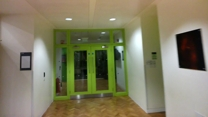
\includegraphics[width=\linewidth]{./gfx/Chapter04/table/5.jpg}
			   \end{minipage}
			        & 54.3  & 49.3 & 58.4 & 1782          & 1326 & 1900 \\ \hline
    C6       & \begin{minipage}{.1\textwidth}
      			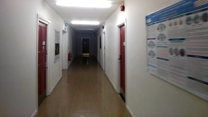
\includegraphics[width=\linewidth]{./gfx/Chapter04/table/6.jpg}
			   \end{minipage}
			        & 55.9  & 55.4 & 56.4 & 1471          & 1180 & 1817 \\ \hline \hline
	\multicolumn{2}{l}{Total}      & \multicolumn{3}{c}{3.042 km} & \multicolumn{3}{c}{90,302 frames} \\ \hline
    \end{tabular}

\end{center}
\end{table}

\subsection{Performance Evaluation}

The methods for a) describing spatial or space-time structure, b) indexing and comparing the data are summarized in Table~\ref{tbl:Methods}. The choice of parameters was selected to allow a) as consistent a combination of methods as possible, allowing fair comparisons of the effect of one type of encoding or spatio-temporal operator to be isolated from others b) to select parameter choices close to other research in the area, e.g.\ for image categorization, the chosen dictionary sizes of $\approx 256$ and $\approx 4000$ words are common. 

\begin{table}
\caption{A summary of the different encoding methods and their relationships to different descriptors. The number of elements of each descriptor is also reported (\textbf{Dim}).}
\label{tbl:Methods}
\small
\centering
    \begin{tabular}{l p{0.5cm} p{0.9cm} p{0.5cm} p{2.5cm} c }
    \hline
    \textbf{Method}              & \textbf{ST} & \textbf{Dense} & \textbf{Dim}  & \textbf{Encoding}      & \textbf{Metric}    \\ \hline
    \multirow{2}{*}{KP\_SIFT} & \multirow{2}{*}{No} & \multirow{2}{*}{No} & \multirow{2}{*}{128}     & HA-4000  &   $\chi^2$    \\ \cline{5-6} 
        ~                   & ~      & ~           & ~      & VLAD-256 & Hellinger \\ \hline
    \multirow{2}{*}{DSIFT} & \multirow{2}{*}{No} & \multirow{2}{*}{Yes} & \multirow{2}{*}{128}     & HA-4000  &   $\chi^2$    \\ \cline{5-6}
    ~                   & ~      & ~           & ~      & VLAD-256 & Hellinger \\ \hline
    \multirow{2}{*}{SF-GABOR} & \multirow{2}{*}{No}               & \multirow{2}{*}{Yes}  & \multirow{2}{*}{136}  & HA-4000  & $\chi^2$      \\  \cline{5-6}
    ~                   & ~      & ~           & ~      & VLAD-256 & Hellinger \\ \hline
    LW-COLOR           & Yes & No & 144           & N/A       \\ \hline
    \multirow{2}{*}{ST\_GABOR}          & \multirow{2}{*}{Yes}              & \multirow{2}{*}{Yes}  & \multirow{2}{*}{221}  & HA-4000  & $\chi^2$      \\  \cline{5-6}
    ~                   & ~      & ~           & ~      & VLAD-256 & Hellinger \\ \hline
    \multirow{2}{*}{ST\_GAUSS}           & \multirow{2}{*}{Yes}              & \multirow{2}{*}{Yes}  & \multirow{2}{*}{136}  & HA-4000  & $\chi^2$      \\  \cline{5-6}
    ~                   & ~      & ~           & ~      & VLAD-256 & Hellinger \\ \hline
    \multirow{2}{*}{HOG3D}               & \multirow{2}{*}{Yes}              & \multirow{2}{*}{Yes} & \multirow{2}{*}{192}   &  HA-4000  & $\chi^2$      \\  \cline{5-6}
    ~                   & ~       & ~          & ~      & VLAD-256 & Hellinger \\ \hline
    \end{tabular}
    \normalsize
\end{table}


\subsubsection{Error distributions}

Error distributions allow us to quantify the accuracy of being able to estimate {\em locations} along physical paths within the RSM dataset described in Section~\ref{sec:Dataset}. To generate the error distributions, we did the following: 

We started by using the kernels calculated in Section~\ref{sec:kernel_encodings}. One kernel is shown in Fig.~\ref{fig:kernel}, where the rows represent each frame from the query pass, and the columns represent each frame from one of the remaining database passes of that corridor. The values of the kernel along a row represent a ``score'' between a query and different database frames given by applying the kernel mapping functions described in \citep{Vedaldi2012} for the $chi^2$ and Hellinger kernel depending on the case. In this experiment, we associated the position of the best match to the query frame, and calculated the error between this and the ground truth $\epsilon$, in m. We used the ground-truth information acquired as described in Section \ref{sec:Dataset}. 

In order to characterise the reliability of such scores, we performed bootstrap estimates of error distributions using 1 million trials. The distribution of the errors gives us a probability density estimate, from which we can get the cumulative distribution function (CDF) $P(x \leq |\epsilon|)$. 

By permuting the paths that are held in the database and randomly selecting queries from the remaining path, we were able to assess the error distributions in localization.  Repeated runs with random selections of groups of frames allowed the variability in these estimates to be obtained, including that due to different numbers of paths and passes being within the database. 

The outcome is shown in Fig.~\ref{fig:CDFall}, where the variability in the lines indicate the range of the results obtained from bootstrapping the observations. The results will be described in the following section.

\begin{figure}[h]
\centering
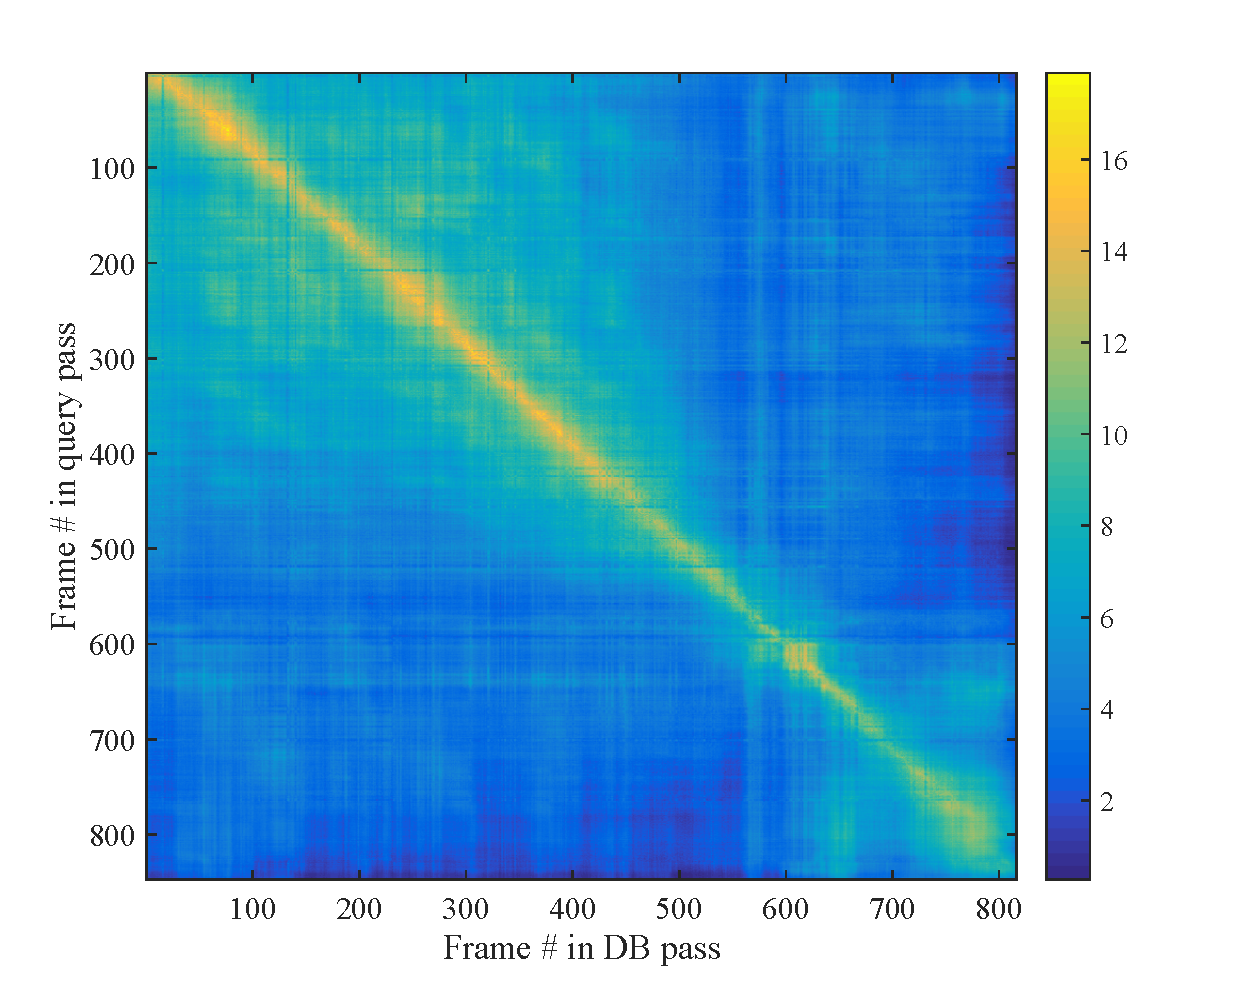
\includegraphics[width=\linewidth]{./gfx/Chapter04/kernel.pdf}
\caption{Example of a $\chi^2$ kernel produced by hard assignment and using the SF\_GABOR descriptors when querying with pass 1 of corridor 2 against a database comprised of passes 2-10.}
\label{fig:kernel}
\end{figure}

If we consider the idea of crowdsourcing journey information from many pedestrian journeys through the same corridors, this approach to evaluating the error makes sense:  all previous journeys could be indexed and held in the database; new journey footage would be submitted as a series of query frames (see Fig.~\ref{fig:pathexample} from Chapter \ref{ch:chapter2}).    

All the results were generated with a downsampled version of the videos at $208 \times 117$ pixels; these are also supplied with the dataset. 




%------------------------------------------------------------------------- 
\section{Results}
\label{sec:ch4results}

We calculated the average absolute positional error (in metres) and the standard deviation of the absolute positional errors across the provided dataset, and these are shown in Table~\ref{Table:summaries}. For these errors, all queries, by a leave-one-out strategy, have been used, but there is otherwise no random sampling of the queries.  Standard deviations of the absolute errors are also provided.  Table~\ref{Table:summaries} also provides the Area-Under-Curve (AUC) values obtained from the CDFs of Fig.~\ref{fig:CDFglobal}.


\begin{figure}[h]
\subfloat[]{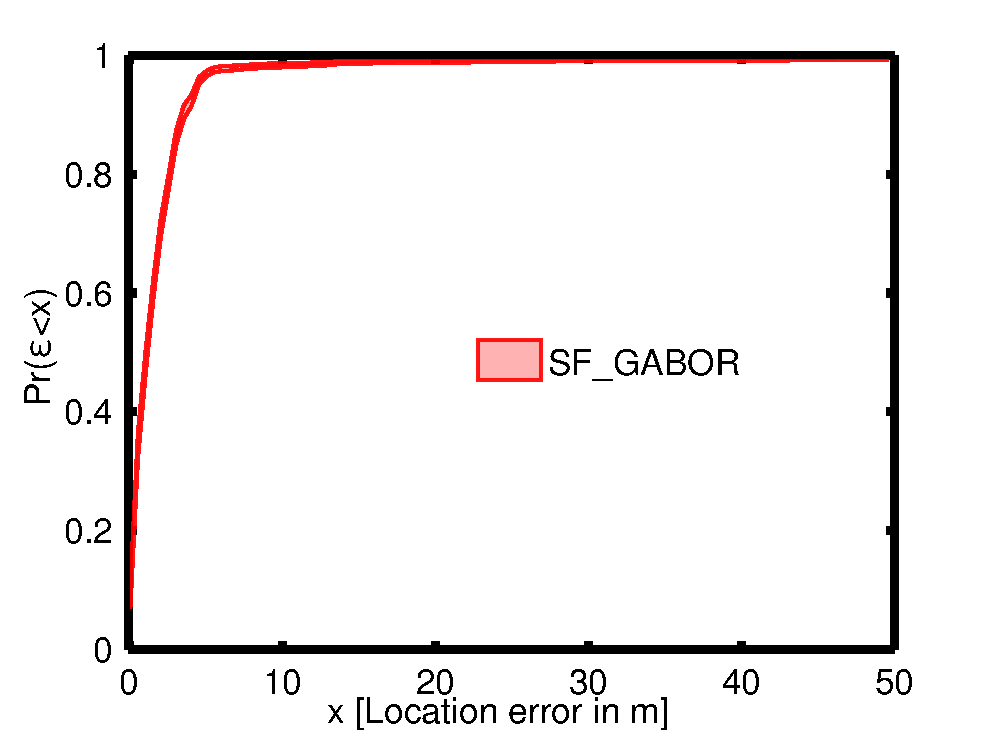
\includegraphics[width=0.33\textwidth]{./gfx/Chapter04/CDF_Figs/SF_GABOR.pdf}}	\subfloat[]{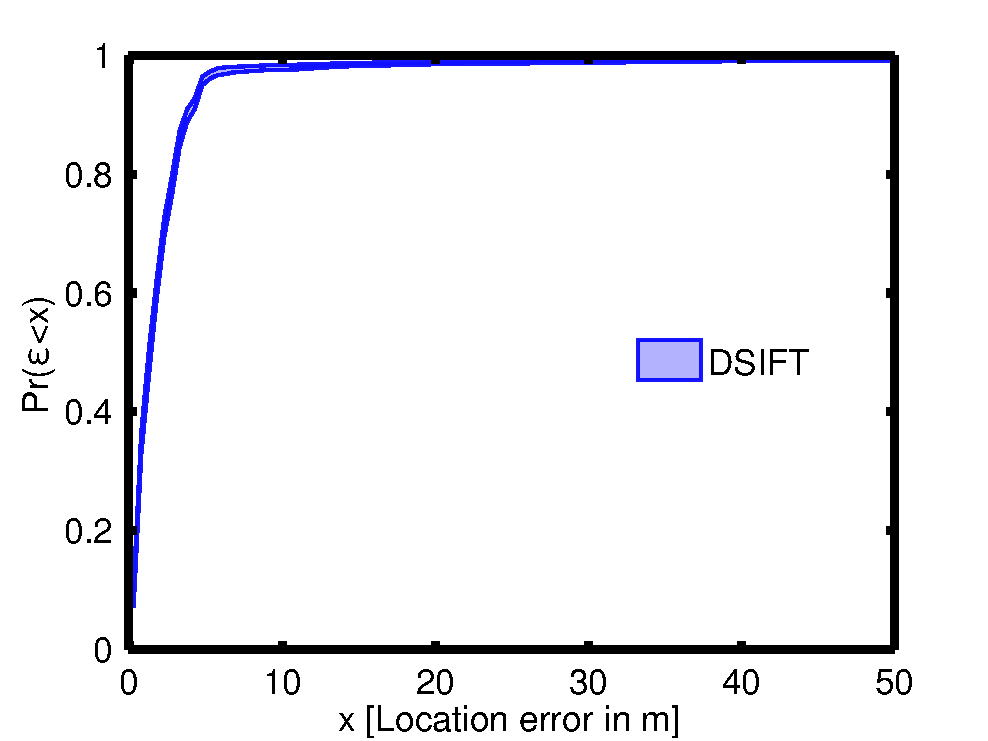
\includegraphics[width=0.33\textwidth]{./gfx/Chapter04/CDF_Figs/DSIFT.pdf}}
\subfloat[]{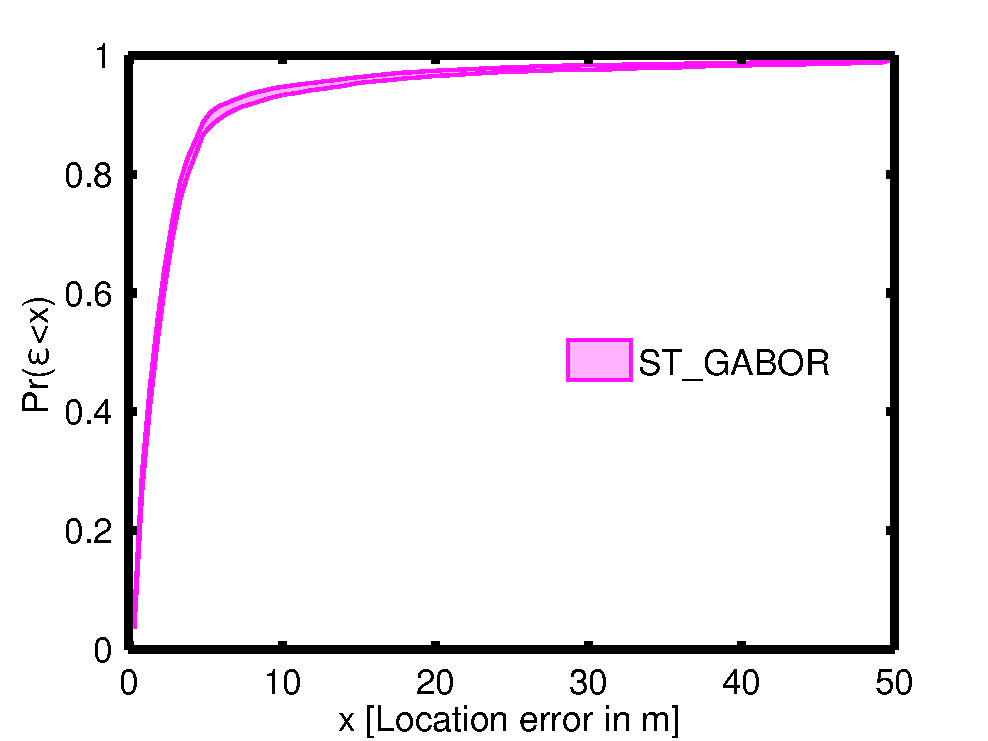
\includegraphics[width=0.33\textwidth]{./gfx/Chapter04/CDF_Figs/ST_GABOR.pdf}}\\
\subfloat[]{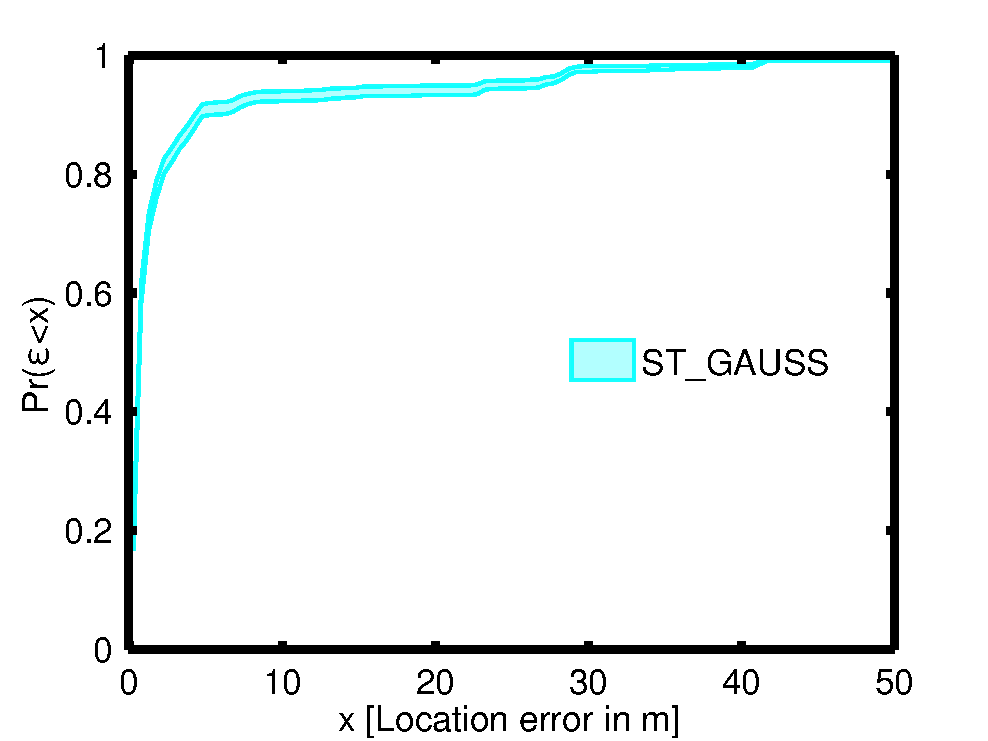
\includegraphics[width=0.33\textwidth]{./gfx/Chapter04/CDF_Figs/ST_GAUSS.pdf}}
\subfloat[]{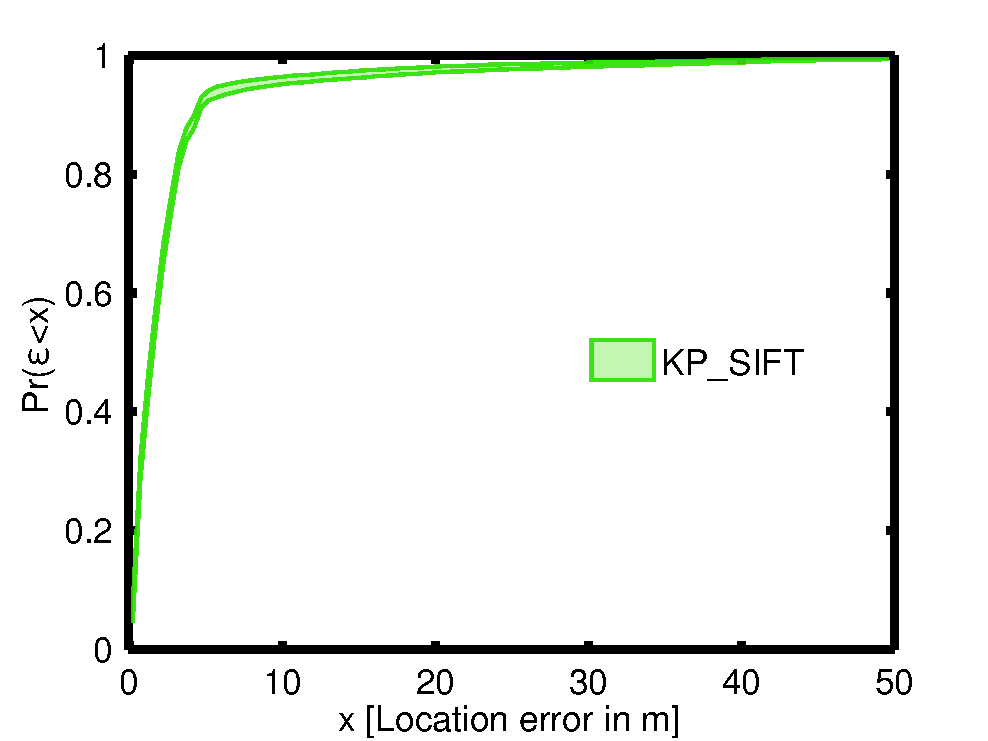
\includegraphics[width=0.33\textwidth]{./gfx/Chapter04/CDF_Figs/KPSIFT.pdf}}
\subfloat[]{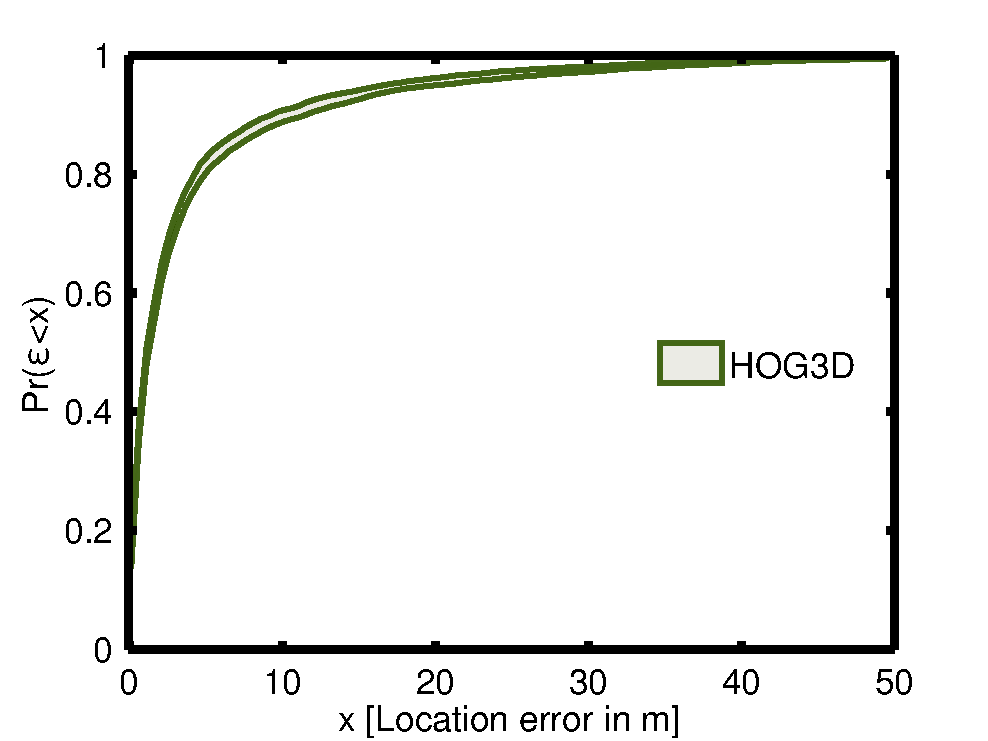
\includegraphics[width=0.33\textwidth]{./gfx/Chapter04/CDF_Figs/HOG3D.pdf}}
\caption{Comparison between the error distributions obtained with the different methods. Note the high reproducibility of the performance results. The origin of the variability within each curve is explained in Section \ref{sec:cdf}}
\label{fig:CDFglobal}
\end{figure}

\begin{figure}
\centering
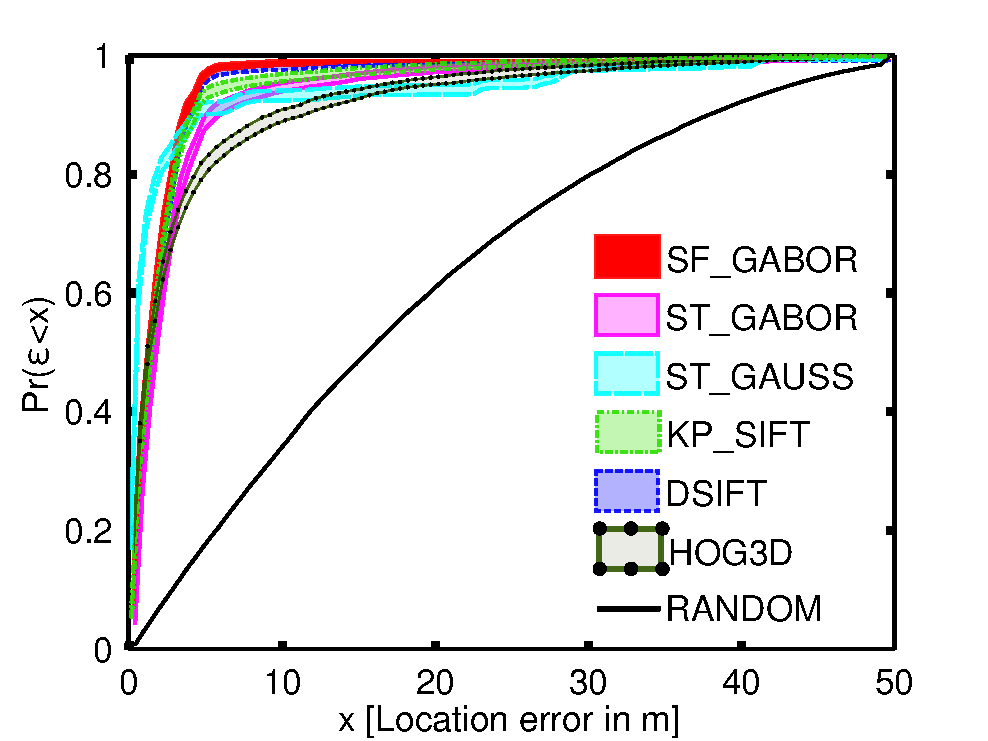
\includegraphics[width=\textwidth]{./gfx/Chapter04/CDF_Figs/all.pdf}
\caption{Comparison between the error distributions obtained with the different methods. The results for a random frame test (RANDOM) were introduced as a ``sanity check''}
\label{fig:CDFall}
\end{figure}



%\begin{figure}[h]
%\begin{center}
%\begin{subfigure}[b]{.6\linewidth}
%\captionsetup{skip=0pt} % local setting for this subfigure
%
%\begin{subfigure}[b]{\linewidth}
%
%	\begin{subfigure}[b]{.45\linewidth}
%	\centering
%	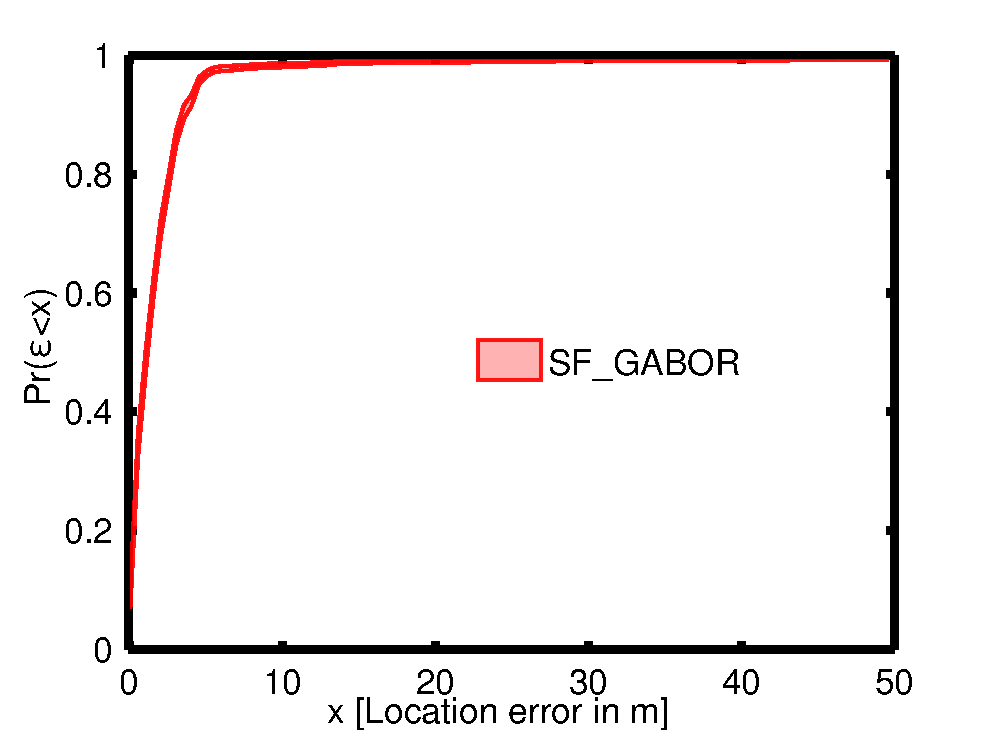
\includegraphics[width=\textwidth]{./gfx/Chapter04/CDF_Figs/SF_GABOR.pdf}\caption{}\label{fig:CDFa}
%	\end{subfigure}
%	\begin{subfigure}[b]{.45\linewidth}
%	\centering
%	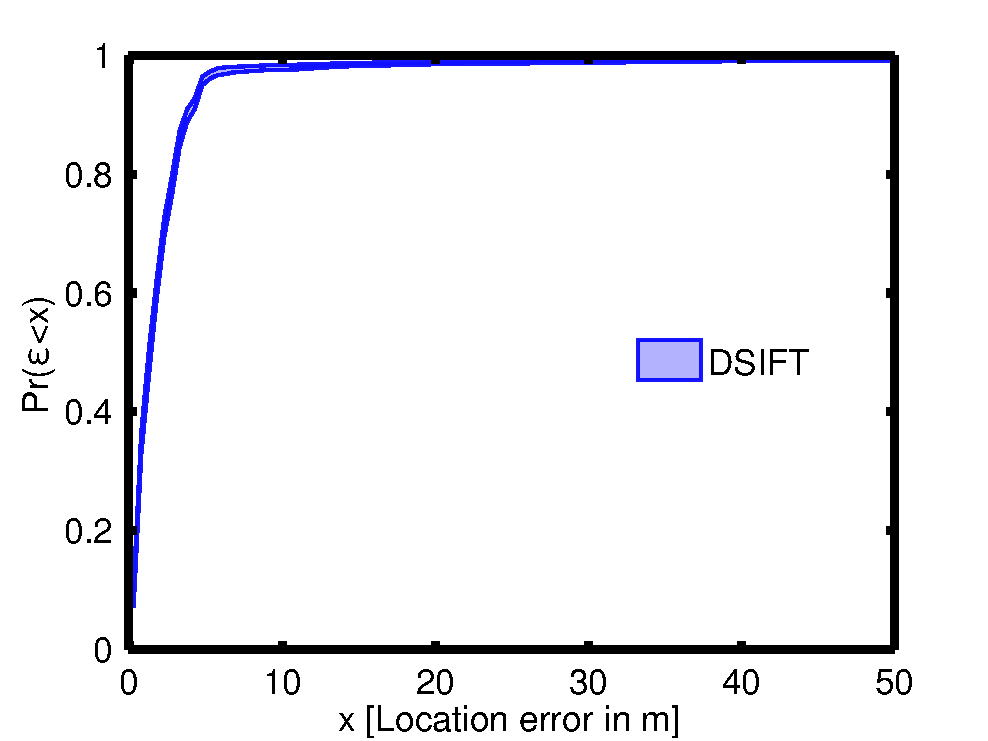
\includegraphics[width=\textwidth]{./gfx/Chapter04/CDF_Figs/DSIFT.pdf}\caption{}\label{fig:CDFb}
%	\end{subfigure}
%	
%\end{subfigure}
%
%
%\begin{subfigure}[b]{\linewidth}
%
%\begin{subfigure}[b]{.45\linewidth}
%\centering
%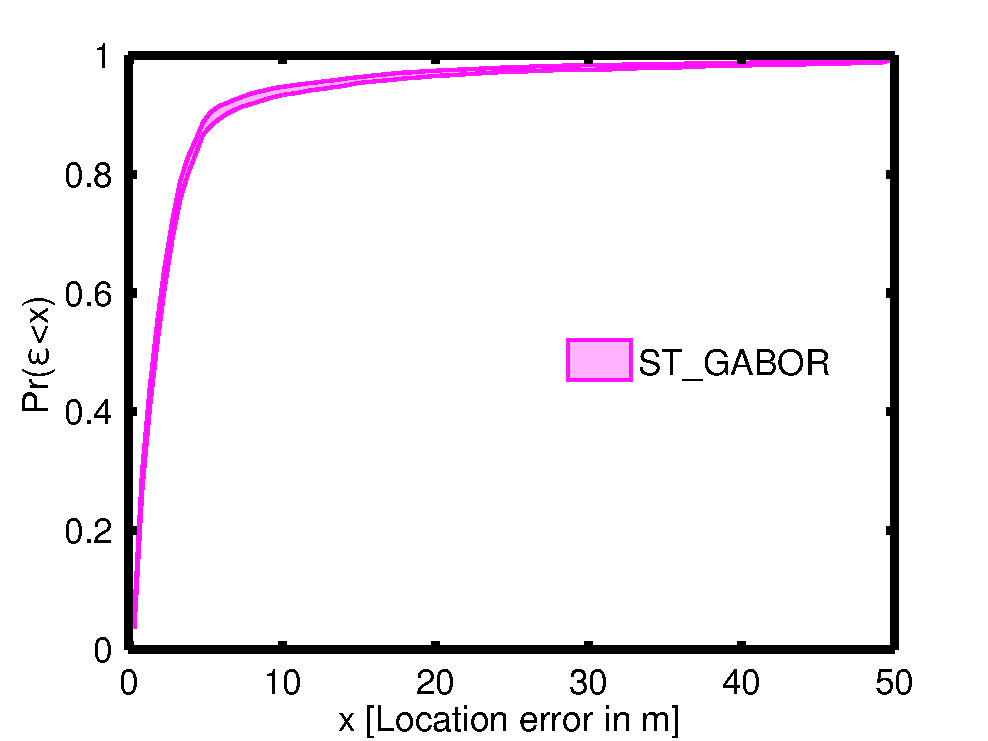
\includegraphics[width=\textwidth]{./gfx/Chapter04/CDF_Figs/ST_GABOR.pdf}\caption{}\label{fig:CDFc}
%\end{subfigure}
%\begin{subfigure}[b]{.45\linewidth}
%\centering
%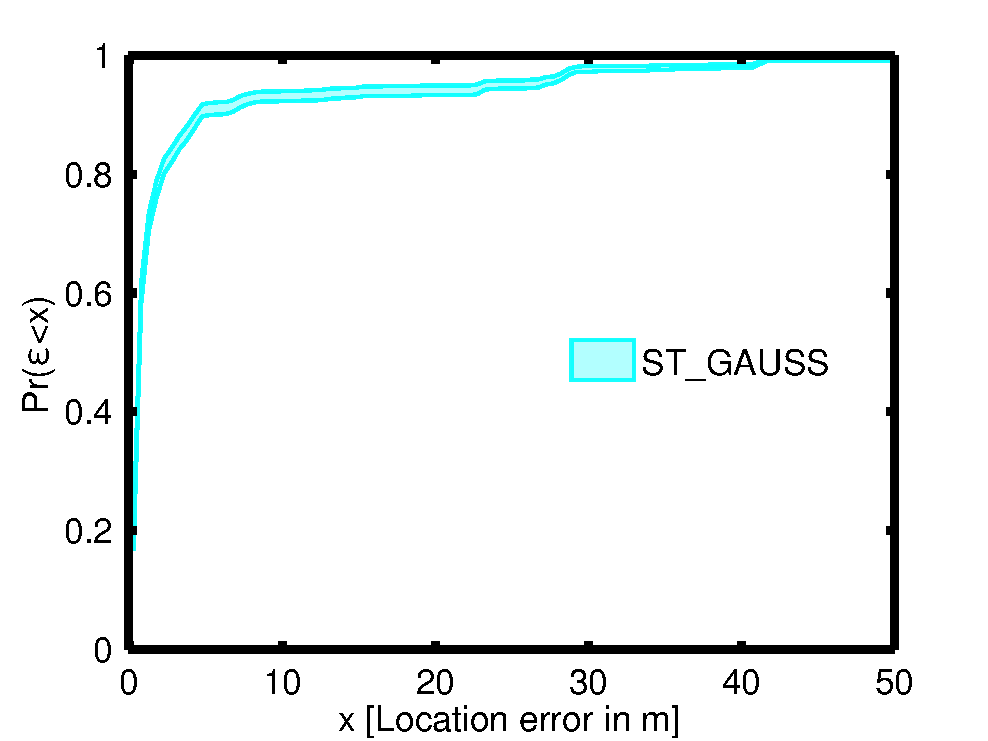
\includegraphics[width=\textwidth]{./gfx/Chapter04/CDF_Figs/ST_GAUSS.pdf}\caption{}\label{fig:CDFd}
%\end{subfigure}
%
%\begin{subfigure}[b]{\linewidth}
%
%	\begin{subfigure}[b]{.45\linewidth}
%	\centering
%	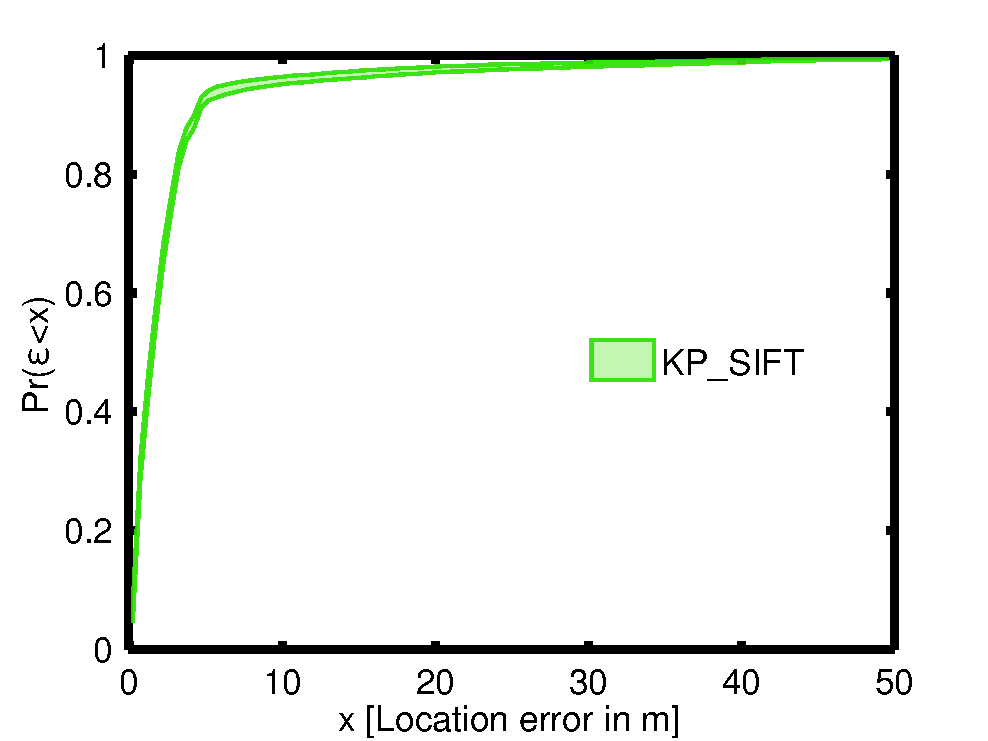
\includegraphics[width=\textwidth]{./gfx/Chapter04/CDF_Figs/KPSIFT.pdf}\caption{}\label{fig:CDFe}
%	\end{subfigure}
%	\begin{subfigure}[b]{.45\linewidth}
%	\centering
%	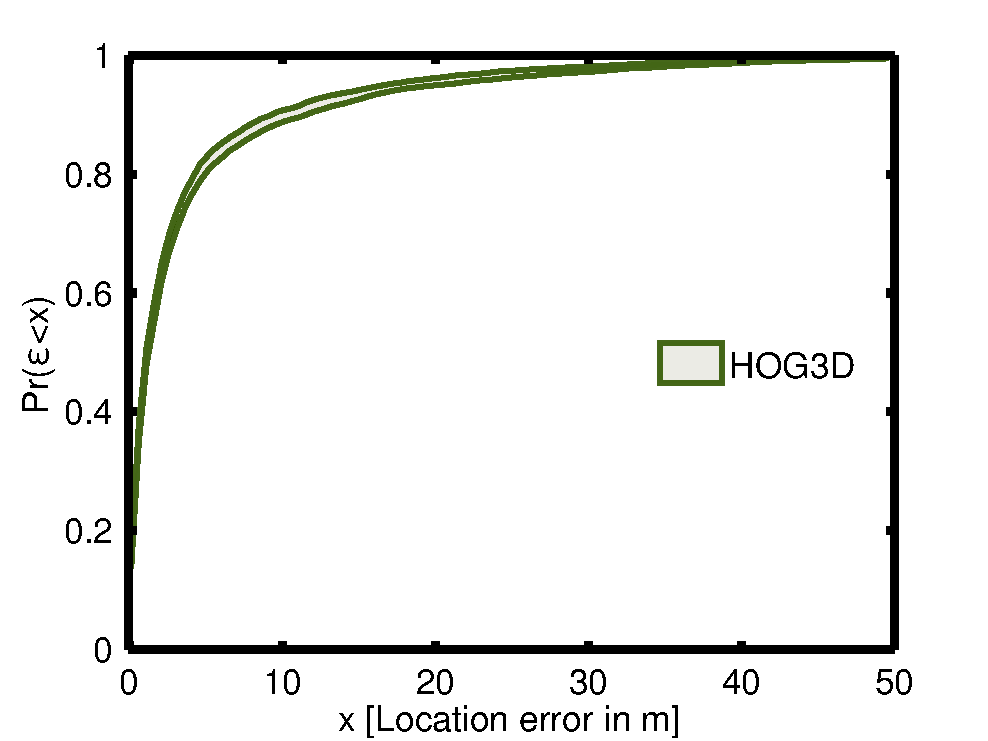
\includegraphics[width=\textwidth]{./gfx/Chapter04/CDF_Figs/HOG3D.pdf}\caption{}\label{fig:CDFf}
%	\end{subfigure}
%	
%\end{subfigure}
%
%\end{subfigure}
%
%\end{subfigure}%
%\begin{subfigure}[b]{.4\linewidth}
%\centering
%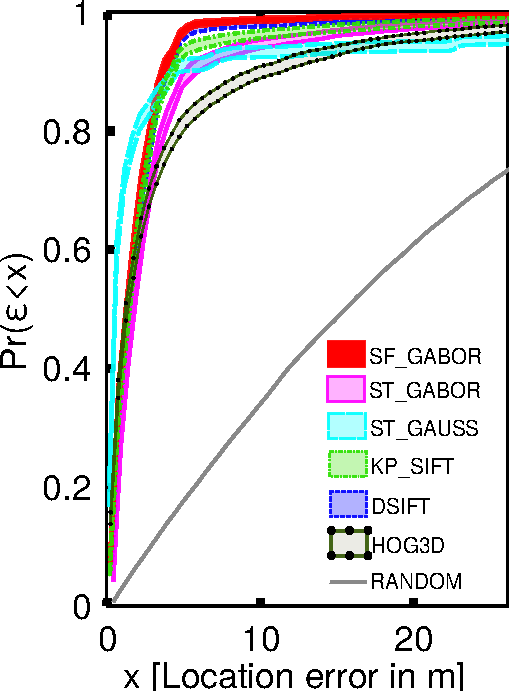
\includegraphics[width=0.95\textwidth]{./gfx/Chapter04/CDF_Figs/CDF_all.pdf}\caption{Comparison between the error distribution obtained with the different methods. The results for a random test (RANDOM) were introduced as a ``sanity check''.}\label{fig:CDFglobal}\label{fig:CDFall}
%\end{subfigure}%
%\caption{Cumulative Distribution Functions of the methods under study.}
%\end{center}
%\end{figure}

\subsection{Localization Error vs Ground-Truth Route Positions}
As described in the previous section, by permuting the database paths and selecting, randomly, queries from the remaining path that was left out in the dictionary creation, we can assess the errors  in localization along each corridor for each pass, and calculate, also, the average error in localization on a per-corridor basis, or per-path basis.  For these, we used the ground-truth information acquired as described in Section \ref{sec:Dataset}.  Fig.~\ref{fig:x_e_vs_gt} provides some examples of the nature of the errors, showing evidence of those locations that are often confused with each other.  As can be seen, for the better method (top trace of Fig.~\ref{fig:x_e_vs_gt}) whilst average errors might be small, there are, occasionally, large errors due to poor matching (middle trace). Errors are significantly worse for queries between different devices (see Fig.~\ref{fig:x_e_vs_gt}(c)). 

\begin{figure}[h!]
\centering
\subfloat[Corridor 3 using Pass 2 acquired with LG Nexus 4. Results for the best spatio-temporal method, ST\_GABOR.]{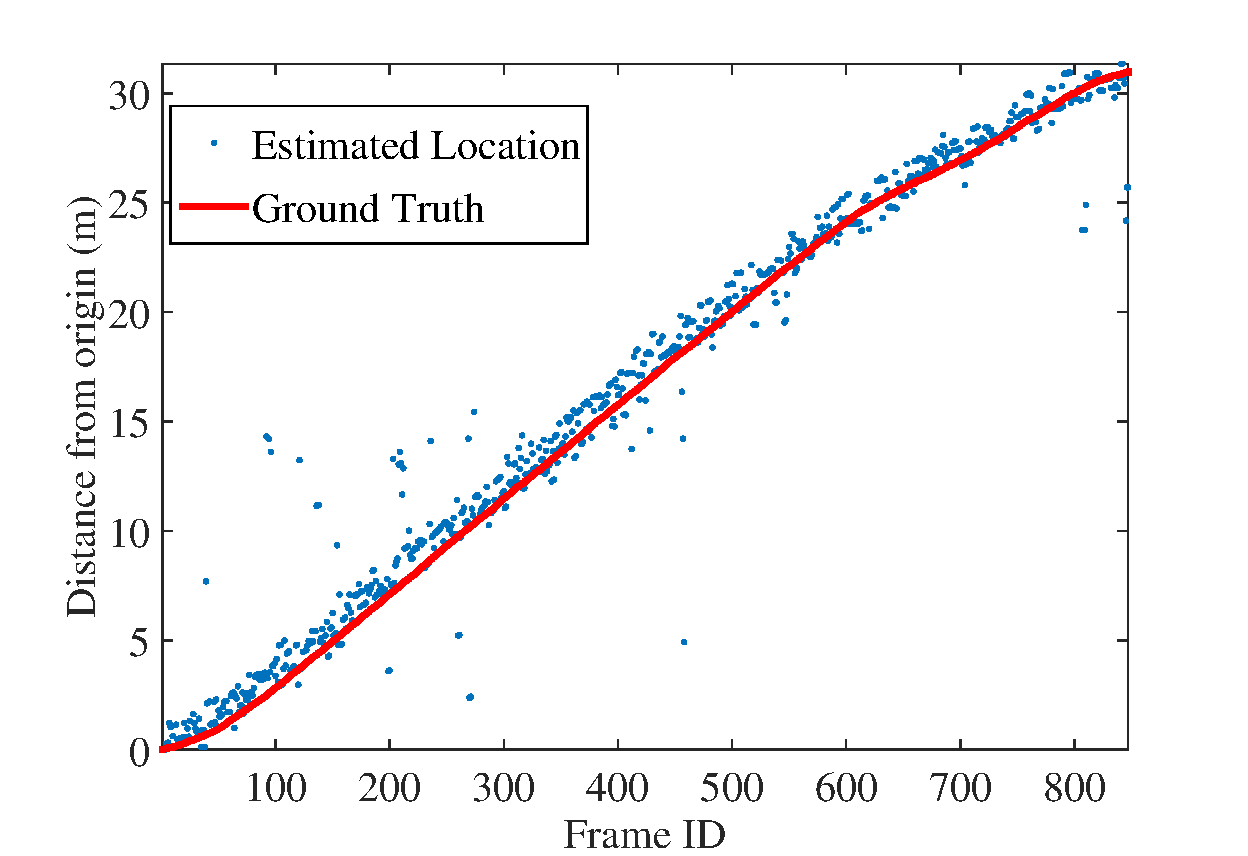
\includegraphics[width=.7\linewidth]{./gfx/Chapter04/xe_vs_x/ST_GABOR_good.pdf}}
\\
\subfloat[Corridor 3 using Pass 6 acquired with Google Glass. Results for the best single-frame method, SF\_GABOR.]{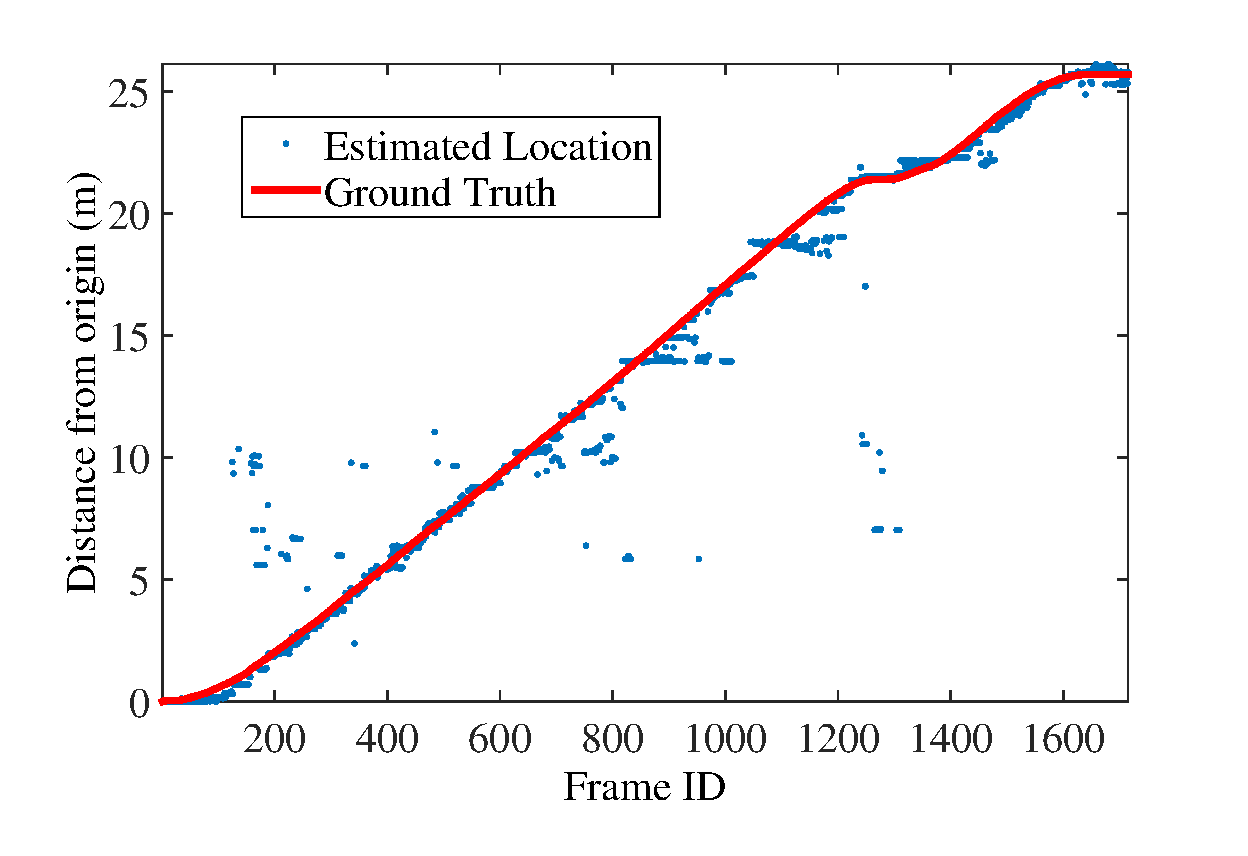
\includegraphics[width=.7\linewidth]{./gfx/Chapter04/xe_vs_x/SF_GABOR_good.pdf}}
\\
\subfloat[Corridor 2 using Pass 6 acquired with Google Glass. Results for the worst overall method, LW\_COLOR.]{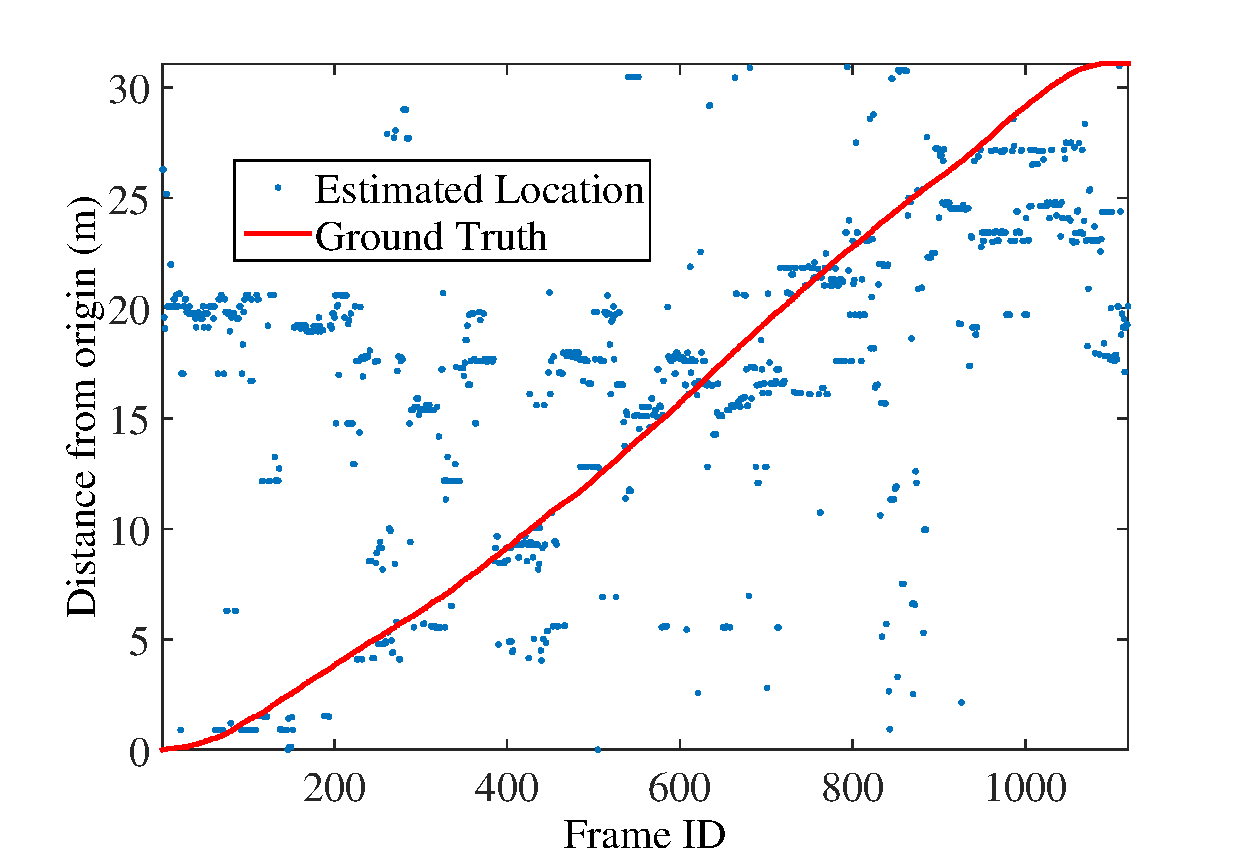
\includegraphics[width=.7\linewidth]{./gfx/Chapter04/xe_vs_x/Lightweight_bad.pdf}}
\caption{Estimated location vs. ground truth. Illustrative examples of good/bad location estimation performance. a) Uses the best descriptor and a single-device dataset, b) uses the best descriptor and a cross-device dataset and c) uses the worst descriptor, and a multiple-device dataset.}
\label{fig:x_e_vs_gt}
\end{figure}


\subsection{Performance Summaries}
We calculated the average of the absolute positional error (in m) and the standard deviation of the absolute positional error in a subset of the complete RSM dataset (Table~\ref{Table:summaries}). We  used a leave-one-journey-out approach (all the frames from an entire journey are excluded from the database).  Using bootstrap sampling, we also estimated the cumulative density functions of the error distributions in position, which are plotted in Fig.~\ref{fig:CDFall}. The variability in these curves is not shown, but is summarized in the last two columns of Table~\ref{Table:summaries} through the area-under-curve (AUC) values. In the best case (SF\_GABOR), AUCs of the order of $~96\%$ would mean errors generally below 2 m; in the worst (HOG3D), AUCs $\approx$ 90\% would mean errors of around 5 m.  These  mean absolute error estimates are obtained as we permute the queries, the dictionary and the paths in the database. 


\begin{table}[!h]
\centering

    \begin{tabular}{ c c c c c }
    \hline
  %  Method   &  Encoding & $\mu_{\epsilon}$ &  $\sigma_{\epsilon}$  & min AUC & max AUC \\ \hline
     \multirow{2}{*}{\bf Method}  & \multicolumn{2}{c}{Error summary (\SI{}{m})} & \multicolumn{2}{c}{AUC (\%)}\\ \cline{2-5}    
    & $\mu_{\epsilon}$ & $\sigma_{\epsilon}$ & Min & Max \\ \hline

    SF\_GABOR       & \textbf{1.59}             & 0.11             & 96.11   & \textbf{96.39}   \\ \hline
    %SF\_GABOR & Hellinger      & 135.1              & 46.5              & 96.29   & 96.71   \\ \hline
	DSIFT           & 1.62              & 0.11  & 95.96   & 96.31   \\ \hline 

	KP\_SIFT           & 2.14              & 0.17  & 94.58   & 95.19   \\ \hline 

	LW\_COLOR           & 3.64              & 1.13  & 91.42   & 92.25   \\ \hline \hline

    %SIFT     & Hellinger      & 132.7              & 41.4              & 94.34   & 94.95   \\ \hline

	% Spatio temporal
	
	ST\_GAUSS        & \textbf{2.11}              & 0.24 & 94.82   & \textbf{95.57}   \\ \hline
    %ST\_GAUSS & Hellinger      & 144.1              & 52.4              & 92.69   & 93.47   \\ \hline
    ST\_GABOR       & 2.54              & 0.19 & 93.90   & 94.44   \\ \hline
    %ST\_GABOR & Hellinger      & 179.5              & 62.3              & 93.98   & 94.60   \\ \hline

    HOG3D         & 4.20              & 1.33              & 90.89   & 91.83   \\ \hline
    %HOG3D    & Hellinger      & 366.5              & 120.3              & 91.49   & 92.37   \\ \hline
    %LW\_COLOR & N/A       & 363.9              & 113.2              & 91.42   & 92.25   \\ \hline
    \end{tabular}


\caption{Summaries of average absolute positional error and standard deviation of positional errors for different descriptor types. $\mu_{\epsilon}$ is the average absolute error, and $\sigma_{\epsilon}$ is the standard deviation of the error in metres. Top: single frame methods. Bottom: spatio-temporal methods.}
\label{Table:summaries}
\end{table}

Note that we did not use any tracking algorithms, and so there is no motion model or estimate of current location given the previous one. As we will describe in Section \ref{sec:slamcomp}, incorporating a particle filter or Kalman filter should reduce the errors, particularly where there are large jumps within small intervals of time. This deliberate choice allows us to evaluate the performance of different descriptor and metric choices independently.

The results show that localization is achieved with good accuracy in terms of CDF and AUC without a large difference between the applied methods, despite the big diversity in their complexity. Absolute errors show significant differences between methods, with average absolute errors in the range of \SI{1.5}{m} to \SI{4.20}{m}. Single frame methods (SF\_GABOR, KP\_SIFT and DSIFT) perform slightly better than spatio-temporal approaches. This is not surprising, as the spatio-temporal methods might be strongly affected by the self motion over fine temporal scales.

In spite of using image retrieval methods in isolation, the attainable accuracy appears to be in line with those of  other methods reviewed in Section~\ref{sec:retrieval}.  However, previously reported methods include tracking, the use of other sensors, or estimates of motion. In this work, no form of tracking was used in estimating position: this was deliberate, in order that we could assess performance in inferring location from the visual data fairly.  Introducing tracking will most possibly improve localization performance, and could reduce query complexity. Yet, tracking often relies on some form of motion model, and for pedestrians carrying or wearing cameras, motion can sometimes be relatively unpredictable. In the next section we will describe the comparison  of our appearance-based approach with SLAM methods, particularly we will reproduce a head-to-head study against large-scale direct monocular SLAM, LSD-SLAM.

%------------------------------------------------------------------------- 
\section{Comparison with state-of-the art SLAM}
\label{sec:slamcomp}
The best performing SLAM method at the time of writing is LSD-SLAM... \td{Decide where to put it}{Relocate here from chapter 5, leave in both places?}


%------------------------------------------------------------------------- 
\section{A visualization of the frame distribution with t-SNE}


t-distributed stochastic neighbor embedding (t-SNE) is a machine learning algorithm for dimensionality reduction developed by Laurens van der Maaten and Geoffrey Hinton.[1] It is a nonlinear dimensionality reduction technique that is particularly well suited for embedding high-dimensional data into a space of two or three dimensions, which can then be visualized in a scatter plot. Specifically, it models each high-dimensional object by a two- or three-dimensional point in such a way that similar objects are modeled by nearby points and dissimilar objects are modeled by distant points.

\begin{figure}
\centering
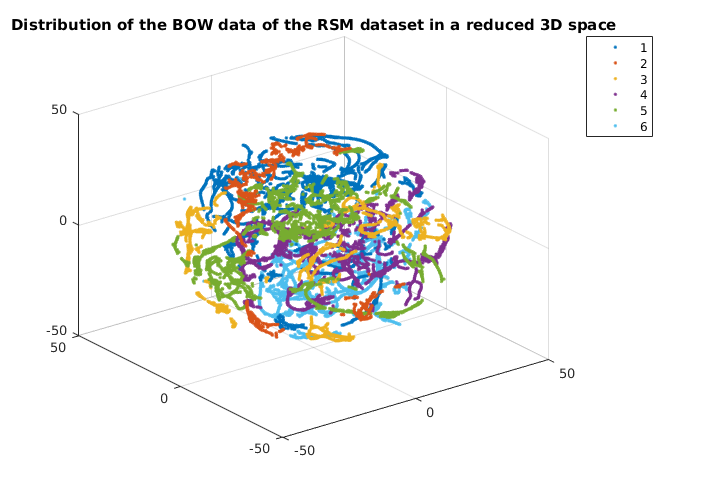
\includegraphics[width=\textwidth]{gfx/Chapter04/visual_paths.png}
\caption{Distribution of the BOW data of the RSM dataset in a reduced 3D space when visualized with t-SNE.}
\label{fig:tsne3d}
\end{figure}

\td{Include}{say that I also changed the distance to cosine one as my values from the histograms are integers}

%------------------------------------------------------------------------- 
\section{Conclusion}

We have presented three main contributions to the topic of indoor localization using visual path matching from wearable and hand-held cameras. We provide an evaluation of six local descriptor methods: three custom designed and three standard image (KP\_SIFT and DSIFT) and video (HOG3D) matching methods as baseline. These local descriptions follow a standard bag-of-words and kernel encoding pipeline. The code for both the local descriptors and for the evaluation pipeline is available on the web page~\cite{Rivera-Rubio2014}. We also make available a large dataset with ground truth of indoor journeys to complete the evaluation framework.

The results show that there is significant localization information in the visual data, and that errors as small as \SI{1.5}{m} over a \SI{50}{m} distance can be achieved, even without tracking. We have reported the results in two ways: a) average absolute positional errors, and b) error distributions, both of which allow image descriptions to be assessed for their localization capability.  The latter could also be used to build a measurement model for inclusion in a Kalman or particle filter  aimed at supporting human ambulatory navigation. 

We plan to introduce tracking in future work. There are, of course, numerous other enhancements that one could make for a system that uses visual data; integration of data from other sensors springs to mind, such as inertial sensing, magnetometers and RSSI.  Although fusing independent and informative data sources would theoretically lead to improvements in performance, we would argue that the methods applied to infer location from each information source should be rigorously tested, both in isolation and as part of an integrated system.  This would help ensure that real-world systems would be somewhat robust to sensor failure. We anticipate that using vision to associate locations in the journeys of several users through their visual paths could play an important role in navigation.

\label{sec:conclusion}


%*****************************************
%*****************************************
%*****************************************
%*****************************************
%*****************************************
